\documentclass{article}
\usepackage{float}
\usepackage{graphicx} % Required for inserting images with \includegraphics command.
\usepackage[hidelinks]{hyperref} % Required in order to use in-page links in the table of contents
                                 % Option "hidelinks" used to hide links border in some pdf reader such as Acrobat Reader.

%Package imported in order to customize cells in tabularx environment. In particular was
%added to allow the use of "\\" syntax inside a table's cell.
\usepackage{makecell}

%Packages and instruction to change scale of sections', subsections' and subsubsections' heads
\usepackage{titlesec}
\usepackage{titlesec}
%Makes sections' contents in bold, and increases their sizes.
\titleformat*{\section}{\Huge\bfseries}
%Same thing as above but for subsections
\titleformat*{\subsection}{\LARGE\bfseries}
%Same thing as above but for subsubsections
\titleformat*{\subsubsection}{\Large\bfseries}

%Instruction used to create a new subsection level (subsubsubsection) in the document
\titleclass{\subsubsubsection}{straight}[\subsection]
%Instructions used to create a new counter (used to count the number of subsubsubsections
%within a subsubsection) for the subsubsubsections and creation of the command to invoke(use) them
\newcounter{subsubsubsection}[subsubsection]
\renewcommand\thesubsubsubsection{\thesubsubsection.\arabic{subsubsubsection}}

%Instruction used to align the new section layer in a correct manner in the table of contents
%Without this subsubsubsections would remain on the same line, creating a mess in the table of
%contents.
\makeatletter

%Instructions to change the scale and font of the subsubsubsections' head
\titleformat{\subsubsubsection}
  {\normalfont\large\bfseries}{\thesubsubsubsection}{1em}{}
\titlespacing*{\subsubsubsection}
{0pt}{3.25ex plus 1ex minus .2ex}{1.5ex plus .2ex}

%Instructions to create the subsubsubsections entries in the table of contents (included the dot line)
\def\toclevel@subsubsubsection{4}
\def\l@subsubsubsection{\@dottedtocline{4}{7em}{4em}}

%Instruction used to restore "@" symbol to "other" instead of a "latter" made by
%\makeatletter command. Just a safety command useful for latex but not of our interest.
\makeatother

%Instructions to set table of contents and sections depth to 4 layers (in order to include even
%subsubsubsections).
\setcounter{secnumdepth}{4}
\setcounter{tocdepth}{4}

%Used in order to have more symbols for itemize lists (in our case the "arrow" symbol in phenomena section)
\usepackage{pifont}

%Used to make the header and footer of each document page
\usepackage{fancyhdr}

%Defines a new style of header and footer
%Defines the content of the header and the footer of the pages of the first section
\fancypagestyle{IntroductionStyle}{
\fancyhf{}
\fancyhead[L]{\textit{\textbf{SECTION 1. INTRODUCTION}}}
\fancyfoot[L]{CKB \quad - \quad \textbf{D}esign \textbf{D}ocument}
\rfoot{\thepage}
\renewcommand{\headrulewidth}{0.4pt}
\renewcommand{\footrulewidth}{0.4pt}
}
%Defines the content of the header and the footer of the pages of the second section
\fancypagestyle{OverallDescriptionStyle}{
\fancyhf{}
\fancyhead[L]{\textit{\textbf{SECTION 2. ARCHITECTURAL DESIGN}}}
\fancyfoot[L]{CKB \quad - \quad \textbf{D}esign \textbf{D}ocument}
\rfoot{\thepage}
\renewcommand{\headrulewidth}{0.4pt}
\renewcommand{\footrulewidth}{0.4pt}
}
%Defines the content of the header and the footer of the pages of the third section
\fancypagestyle{SpecificRequirementsStyle}{
\fancyhf{}
\fancyhead[L]{\textit{\textbf{SECTION 3. USER INTERFACE DESING}}}
\fancyfoot[L]{CKB \quad - \quad \textbf{D}esign \textbf{D}ocument}
\rfoot{\thepage}
\renewcommand{\headrulewidth}{0.4pt}
\renewcommand{\footrulewidth}{0.4pt}
}
%Defines the content of the header and the footer of the pages of the fourth section
\fancypagestyle{FormalAnalysisAlloyStyle}{
\fancyhf{}
\fancyhead[L]{\textit{\textbf{SECTION 4. REQUIREMENTS TRACEABILITY}}}
\fancyfoot[L]{CKB \quad - \quad \textbf{D}esign \textbf{D}ocument}
\rfoot{\thepage}
\renewcommand{\headrulewidth}{0.4pt}
\renewcommand{\footrulewidth}{0.4pt}
}
%Defines the content of the header and the footer of the pages of the fifth section
\fancypagestyle{EffortSpentStyle}{
\fancyhf{}
\fancyhead[L]{\textit{\textbf{SECTION 5. IMPLEMENTATION, INTEGRATION, TEST PLAN}}}
\fancyfoot[L]{CKB \quad - \quad \textbf{D}esign \textbf{D}ocument}
\rfoot{\thepage}
\renewcommand{\headrulewidth}{0.4pt}
\renewcommand{\footrulewidth}{0.4pt}
}
%Defines the content of the header and the footer of the pages of the sixth section
\fancypagestyle{ReferencesStyle}{
\fancyhf{}
\fancyhead[L]{\textit{\textbf{SECTION 6. EFFORT SPENT}}}
\fancyfoot[L]{CKB \quad - \quad \textbf{D}esign \textbf{D}ocument}
\rfoot{\thepage}
\renewcommand{\headrulewidth}{0.4pt}
\renewcommand{\footrulewidth}{0.4pt}
}
%Defines the content of the header and the footer of the pages of the seventh section
\fancypagestyle{ReferencesStyle}{
\fancyhf{}
\fancyhead[L]{\textit{\textbf{SECTION 7. REFERENCES}}}
\fancyfoot[L]{CKB \quad - \quad \textbf{D}esign \textbf{D}ocument}
\rfoot{\thepage}
\renewcommand{\headrulewidth}{0.4pt}
\renewcommand{\footrulewidth}{0.4pt}
}

%Used to handle table width and split tables across different pages
\usepackage{xltabular}
%Change space between table columns
\setlength{\tabcolsep}{18pt}

%Command used to create a new column type whose background is lightgray colored
\usepackage{xcolor,colortbl}
\definecolor{LightGray}{gray}{0.85}
\newcolumntype{g}{>{\columncolor{LightGray}}c}


%Set the default path of images (used in includegraphics command)
\graphicspath{ {images/} }

\title{\Huge{\textbf{Design Document}}}
\author{\Large{Francesco Spangaro - Tosetti Luca - Francesco Riccardi}}
\date{07 January 2024}

\begin{document}

\maketitle

\begin{figure}[h]
    \centering
    
\includegraphics[scale=0.6]{politecnico-di-milano-logo.png}
\end{figure}

\vspace*{1cm}
\begin{center}
      \Large{\textbf{Prof.}} \\
      \Large{\textbf{Matteo Camilli}}
\end{center}
\vspace*{1cm}

\begin{center}
      \large{Version 0.2} \\
      \large{Academic Year 2023 - 2024}
\end{center}
\newpage
\tableofcontents


\pagestyle{IntroductionStyle}

\section{Introduction}
\subsection{Purpose}
The purpose of this document is to provide an exhausting and implementative
description of the platform that will be implemented (CKB platform).
In particular the document is focused on the description of the architectural styles and decisions
that will be adopted, the modules that compose the platform and their interfaces.
The document will contains also several details regarding the deployment choices,
the runtime view of the core functionalites of the platform that will be used in it.
The document contains some mockups of the user interface design.
The document also covers the implementation, integration and testing
processes required to implement correctly the CKB platform.
\subsection{Scope}
CodeKataBattle (CKB) is a platform which aims to give to Educators an easy-to-use experience, and let
them propose homework and/or lessons in a new and fresh way.
The main goal of the platform is to give the Students the possibility to improve and acquire new software
developing skills by particpating to several battles in as many tournaments.
The platform let Educators of the Students to create such tournaments and battles within them
in order to challenge the Students to upload the best possible solution to the battle's
problem. That solution will be then automatically evaluated by the platform which will give it a score,
and eventually even by the Educator who created the battle, and will be associated to it a proper score.
The platform also allow Educators to add several recognition badges for the work done by the students.
This badges can be personalized by the Educators themselves.
\\ \\
From the architectural point of view we have decided to adopt a 4-Tier Client-Server architecture combined
with a MSA server side, in addition to a MVC software architectural choice.
\subsection{Definitions, acronyms, abbreviations}
\subsubsection{Definitions}
{\renewcommand{\arraystretch}{1.5}
%\textwidth used to set table's width according to text's width of the page
%">{\raggedright\arraybackslash} c" used to align to the right the column c
%"X" column tag creates a paragraph-like column whose width automatically expands so that the declared width of the environment is filled
\begin{xltabular}{\textwidth}{ >{\raggedright\arraybackslash}c >{\raggedright\arraybackslash}X }
    \hline
    \textbf{Term} & \textbf{Definition} \\
    \hline

    \endfirsthead   %Everything above is used as "head" (first row) of
    %the table in the page where it is placed

    \hline
    \textbf{Term} & \textbf{Definition} \\
    \hline

    \endhead    %Everything above is used as "head" (first row) of the
    %splitted parts of the table in the pages different from
    %the one in which the table was originally placed

    \endfoot    %Everything above is used as "foot" (last row) of the
    %splitted parts of the table in the pages different from
    %the last one in which the table appear

    \endlastfoot    %Everything above is used as "foot" (last row) of the
    %table in the page where it appears last.

    \textit{4-Tier Architecture} & $\rightarrow$ A 4-Tier architecture in the field of informatic systems, very simply
    a software and hardware architecture in which a running application/platform is divided in four different modules
    or also called "layers" which usually are: Presentation Layer, WebServer layer, Logic Layer, Data Layer. \\
    \textit{Presentation Layer} & $\rightarrow$ The top layer of the 4-Tier architecture. It takes care of the interaction
    between the user and the application.\\
    \textit{WebServer Layer} & $\rightarrow$ The second layer of the 4-Tier architecture. It takes care of handling the requests
    sent by the users throught a browser application. \\
    \textit{Logic Layer} & $\rightarrow$ The third layer of the 4-Tier architecture. It takes care of implementing the real
    application logic that allows to the application/platform to actually work. \\
    \textit{Data Layer} & $\rightarrow$ The bottom layer of the 4-Tier architecture. It takes care of all the data generated
    by the users or the application, and with which the application itself has to interact. The interactions
    can include queries, updates, deletions, ... \\
    \textit{Microservice architecture} & $\rightarrow$ An architectural style that consist in the creation of an
    application/platform as a suite of small services, each one handling a part of the business logic of the application
    and that comunicates with each other throught lightweight protocols (such as HTTP). \\
    \textit{Model-View-Controller} & $\rightarrow$ An architectural pattern used to develop the
    software logic of an application. This pattern consist in dividing the application in three
    different parts: View, Model and Controller. \\
    \textit{View} & $\rightarrow$ Part of the MVC pattern which takes care of the visualization of the
    data contained in the model and the interaction with the user. \\
    \textit{Controller} & $\rightarrow$ Part of the MVC pattern that receives commands from the user, and execute them
    by modifying the View and/or Model parts. \\
    \textit{Model} & $\rightarrow$ Part of the MVC pattern that gives to the Controller part, the
    methods to access the application's data and to modify them.
\end{xltabular}

\subsubsection{Acronyms}
\begin{xltabular}{\textwidth}{ >{\raggedright\arraybackslash}c >{\raggedright\arraybackslash}X }
    \hline
    \textbf{Acronym} & \textbf{Meaning} \\
    \hline

    \endfirsthead

    \hline
    \textbf{Acronym} & \textbf{Meaning} \\
    \hline

    \endhead
    \endfoot
    \endlastfoot

    \textit{MSA} & $\rightarrow$ MicroServices Architecture\\
    \textit{MVC} & $\rightarrow$ Model-View-Controller\\
    \textit{RASD} & $\rightarrow$ Requirement Analysis and Specification Document\\
    \textit{DD} & $\rightarrow$ Design Document\\
    \textit{CKB} & $\rightarrow$ CodeKataBattle\\
    \textit{} & $\rightarrow$ \\
\end{xltabular}


\subsubsection{Abbreviations}
\begin{xltabular}{\textwidth}{ >{\raggedright\arraybackslash}c >{\raggedright\arraybackslash}X }
    \hline
    \textbf{Abbreviation} & \textbf{Meaning} \\
    \hline

    \endfirsthead

    \hline
    \textbf{Abbreviation} & \textbf{Meaning} \\
    \hline

    \endhead
    \endfoot
    \endlastfoot

    \textit{e.g.} & $\rightarrow$ Exempli gratia, latin phrase meaning "for example".
    \\
    \textit{i.e} & $\rightarrow$ Id Est, lating phrase meaning "that is".
    \\
    \textit{} & $\rightarrow$
    \\
    \textit{} & $\rightarrow$
    \\
    \textit{} & $\rightarrow$
    \\
\end{xltabular}
\subsection{Revision history}
\begin{itemize}
    \item **Placeholder data**: version 1.0
\end{itemize}

\subsection{Reference documents}
UML official specification $\rightarrow$ \url{https://www.omg.org/spec/UML}
\\ \\
Sequence diagrams specification $\rightarrow$ \url{https://www.uml-diagrams.org/sequence-diagrams.html}
\\ \\
Component diagrams specification $\rightarrow$ \url{https://creately.com/blog/software-teams/component-diagram-tutorial/}
\\ \\
Deployment diagrams specification $\rightarrow$ \url{https://pubs.opengroup.org/architecture/archimate32-doc.singlepage/}
\subsection{Document structure}
\begin{itemize}
    \item \textbf{\textit{Section 1: Introduction}} \\
          This section offers a brief description of the problem and the platform/application that will be developed in order to resolve it.
          It describes the major purpose of this document, a very brief recap of the domain which is
          described in detail in the RASD document.
          In addition, in this section are inserted definitions, acronyms and abbreviations used in the document,
          its revision history and refereced documents or web pages.
    \item \textbf{\textit{Section 2: Architectural Design}} \\
          This section is the main part of the document. It describes the architectures used to
          realize the platform, the CKB platform's components, its interfaces, its deployment
          structure and finally its runtime behaviour.
          All these aspects are described through several diagrams such as:
          component diagrams, class diagrams, deployment diagrams and other
          generic diagrams which are used to give a representation of main and most important
          features of the platform.
    \item \textbf{\textit{Section 3: User interface design}} \\
          This section describes the user interface design of the platform.
          It contains several mockups of the interface that the Educators and
          Students will find when they access to the platform. The presented mockups
          refers to the client-side experience throught an appropriate browser application.
    \item \textbf{\textit{Section 4: Requirements traceability}} \\
          This section describe the connection between the RASD and DD document,
          by providing a complete map of the requirements and goals expressed in the RASD
          to the modules presented in this document.
    \item \textbf{\textit{Section 5: Implementation, Integration \& Test plan}} \\
          This section describes the plan followed for implementing, testing and
          integrating the platform's components, the order in which
          these operations are performed and what they generate.
    \item \textbf{\textit{Section 6: Effort spent}} \\
          This section contains all the information about the time spent by each group member
          in order to complete this document and its division by each section of the document.
\end{itemize}
\section{Architectural Design}
\subsection{Overview: High-level components and interactions}
To ensure high maintainability, security and reliability, the service is structured by following the four-tier architecture model.
Figure 1. shows how the tiers are divided, and what are the relations between each tier of the system.
\begin{figure}[H]
    \centering
    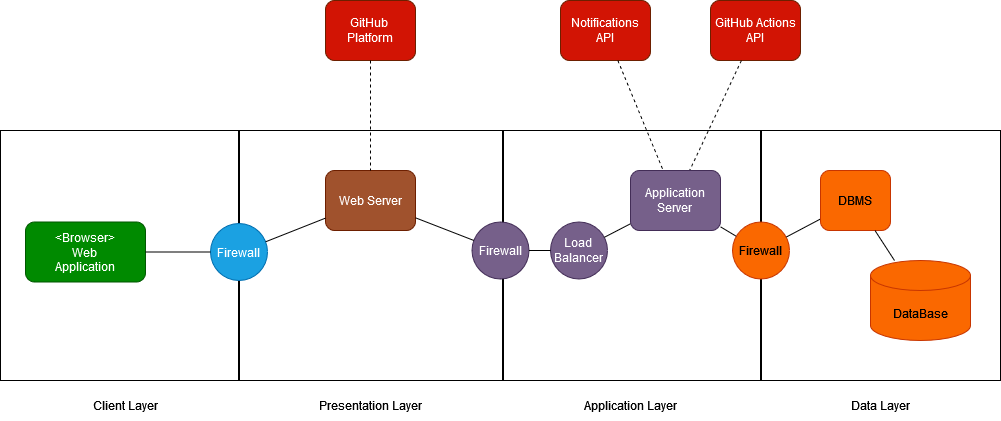
\includegraphics[scale=0.35]{images/FourTierApplication.png}
    \caption{Four-tier architecture}
    \label{fig:Figure 1}
\end{figure}
\noindent
The main components are: \\ \\
\begin{itemize}
\item \textbf{Web Application:} The web application allows users to connect to the platform's services. The web application can be accessed by any device
that is connected to the internet and can browse the web. Students and Educators will have different views of the web application, because they have
different parameters that they can view and manage. \\ \\
\item \textbf{Web Server:} The web server is what manages the web application. It is connected directly to the GitHub Platform to give Educators the possibility
of seeing their Students' uploaded solutions. It is connected to the GitHub platform to also give Students the possibility of seeing their
solutions uploaded to the platform in real time. It is the main container for the JavaScript and general backend code for the platform.
The web server is connected to the Application server because it needs to be automatically updated when new grades for Students' solutions are generated
by the platform. \\ \\
\item \textbf{Application Server:} The application server is the main backend of the CKB Platform. It contains all the code needed for th eplatform to run
smoothly and without interruptions. It contains the logic needed to answer the API requests made by the users to the platform. It
automatically evaluates Students' solutions proposed via the GitHub platform and uploads the new grade to the web server. \\ \\
\item \textbf{DBMS:} The DBMS is the main interpreter between the CKB platform and the data stored onto the database. \\ \\
\item \textbf{DataBase:} The database stores all the information needed by the application. \\ \\
\item \textbf{External Services:} These services provide informations and funtionalities that the CKB platform alone could not provide.
These funtionalities include a \textit{GitHub actions API} that notifies the platform of the upload of a new Student's solution, a \textit{notification API}
that notify Students when a new tournament or a new battle in a tournament they are subscribed to is created and a connection to the \textit{GitHub platform}
since the code needs to be uploaded from the GitHub platform to the CKB platform automatically. \\
\end{itemize}
\subsection{Component view}
\begin{figure}[H]
    \centering
    \hspace*{-4.1cm}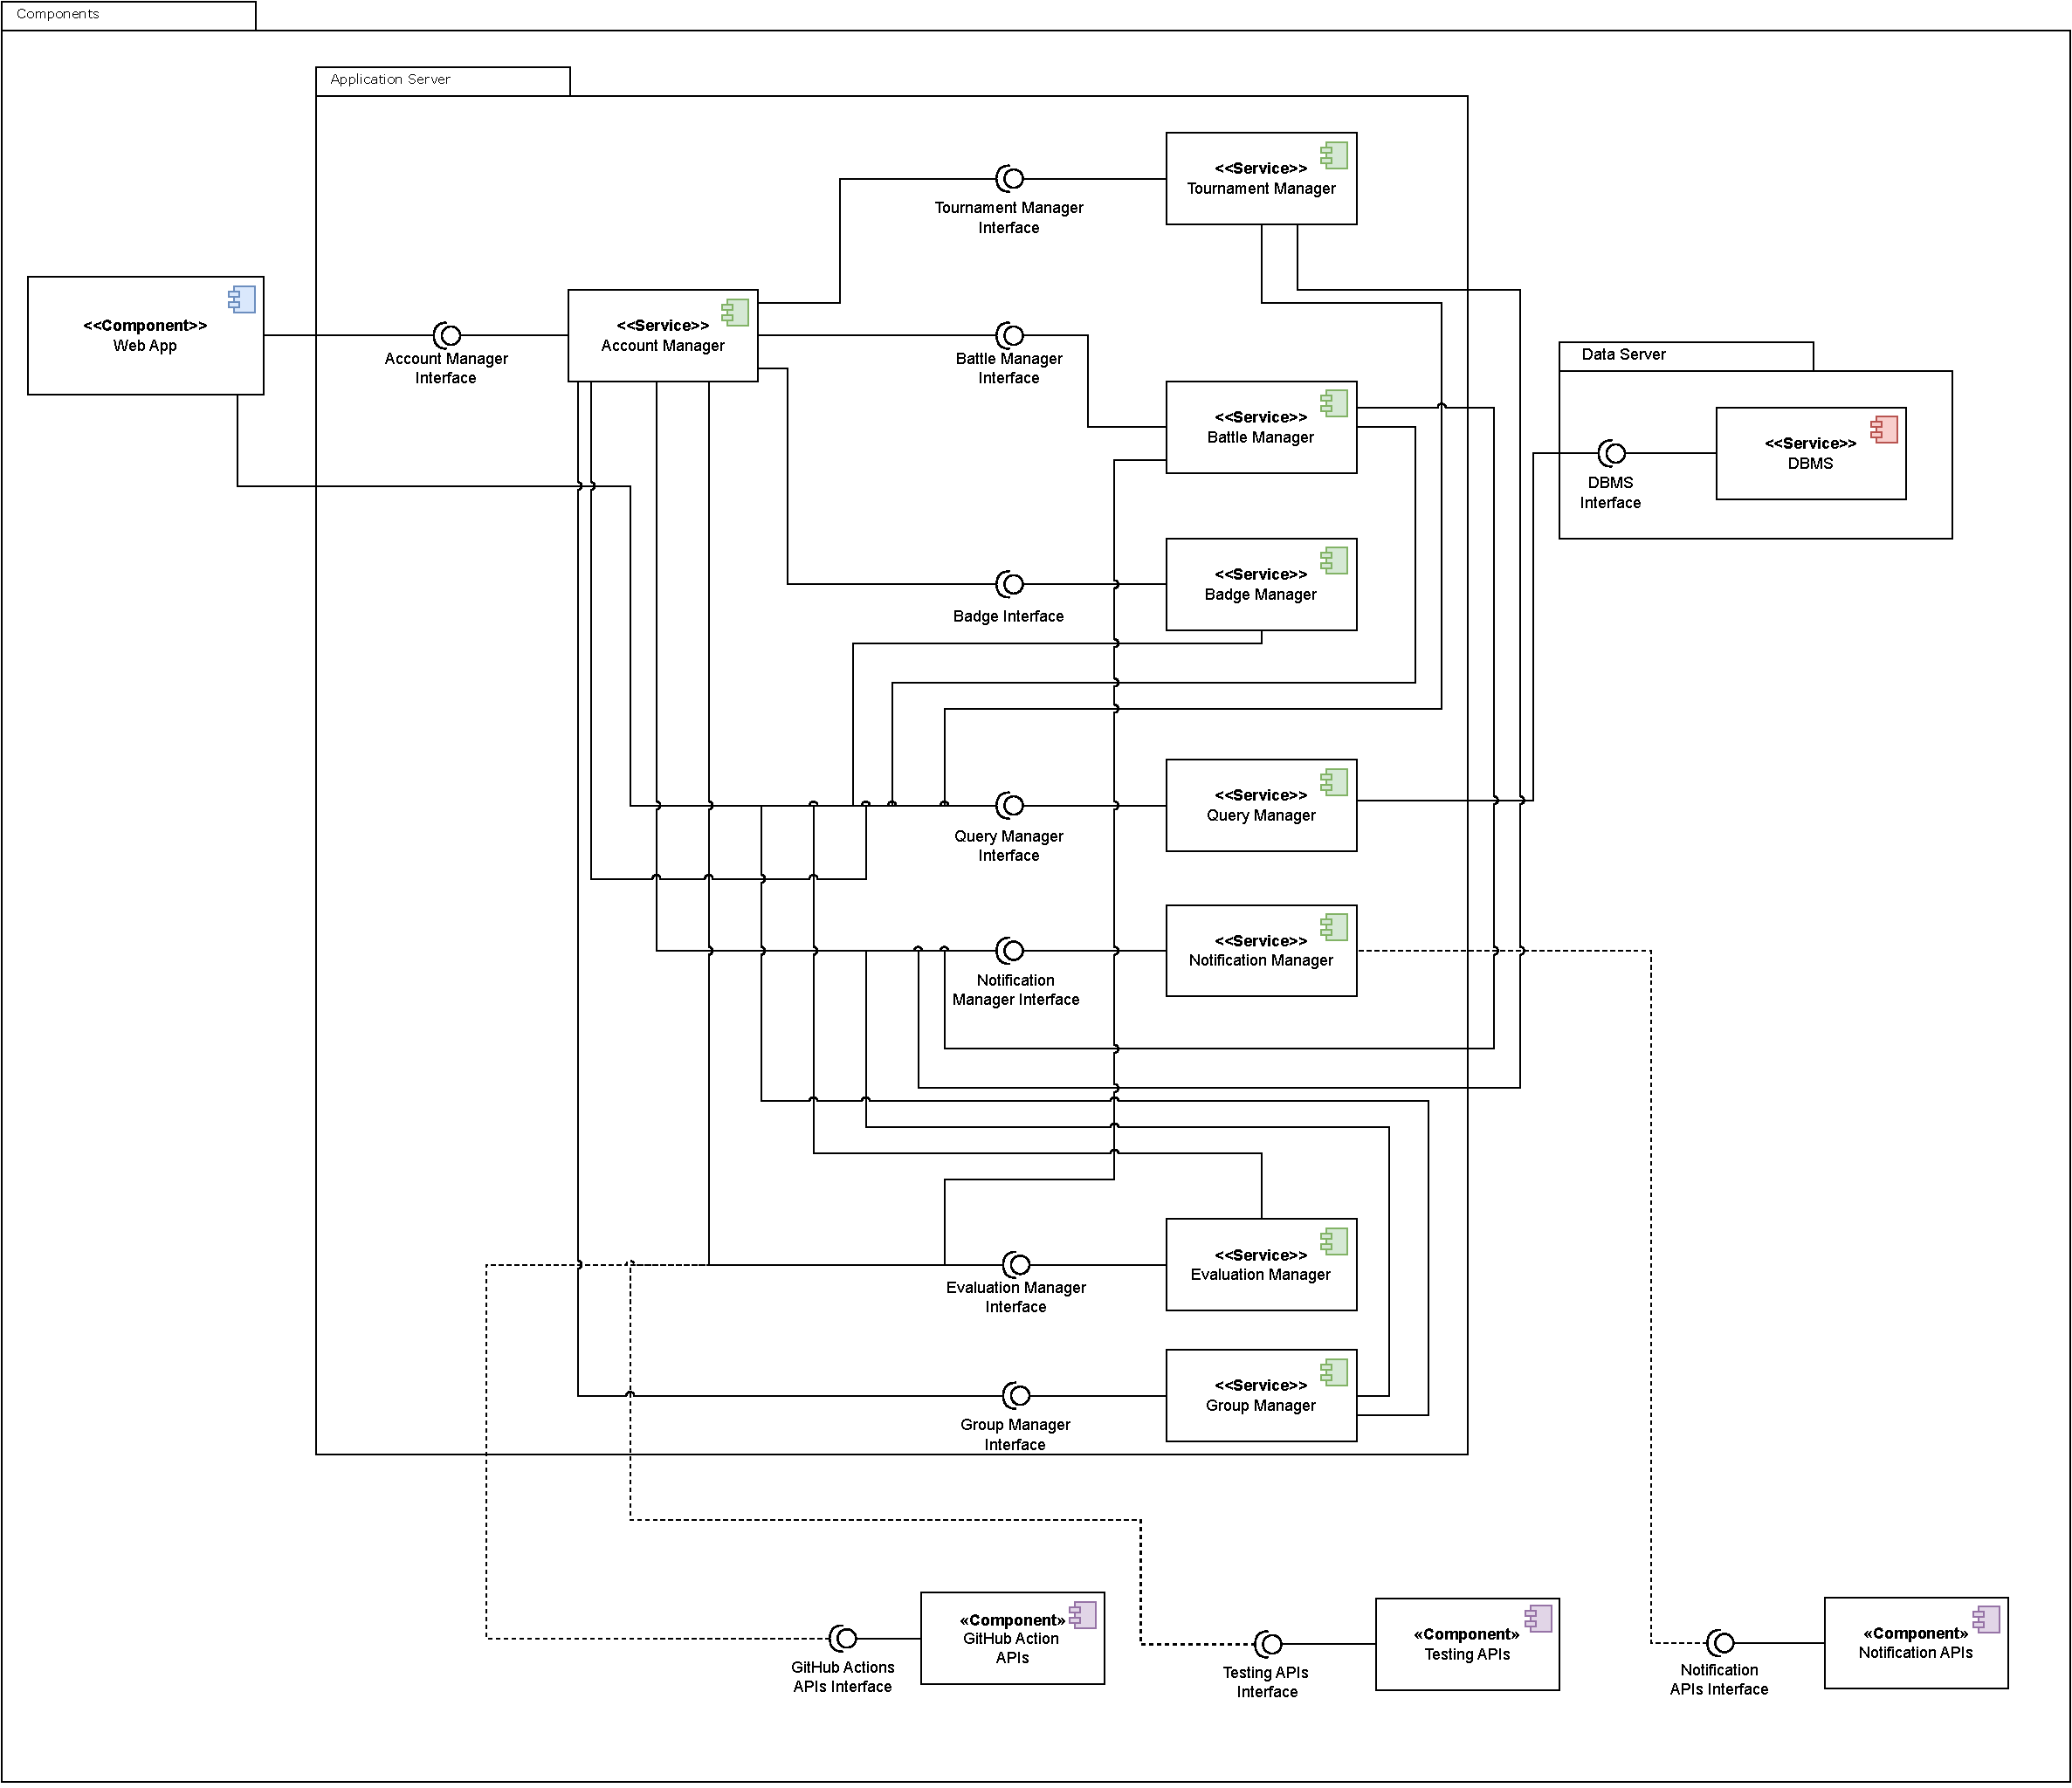
\includegraphics[scale=0.5]{images/ComponentView.pdf}
    \caption{Component diagram}
    \label{fig:componentView}
\end{figure}
In Figure 2 we can see a more detailed diagram, representing all the components previously described.
The Web App is what Students and Educator connect to via their web browsers.
It collects all of the Students' and Educators' requests, forwards them to the right service or component and sends back different responses.
\\
\begin{itemize}
\item \textbf{Account Manager:} The Account Manager is the module that handles the client's logins and creates the session. 
It checks the client's data and permissions and creates a session with the data he collects. This data session is what is used by the other services and
interfaces to grant the user different permission levels. \\
E.G. A Student can use the Tournament Manager differently from an Educator, since the Student can subscribe to a tournament and see the battles it contains,
while an Educator can use the Interface to manage the tournament.\\
\item \textbf{Tournament Manager:} The Tournament Manager is the module that lets Educators create and manage tournaments and it lets them grant permission
to create battles in their tournaments to other Educators. \\
It lets Students visualise all open tournaments and subscribe to each tournament they want. \\
\item \textbf{Battle Manager:} The Battle Manager is the module that lets Educators create and manage battles within their tournaments, or within tournaments
for which they have been granted permission to create and manage battles from the tournament's creator. \\
It lets Students visualise the battles in tournaments they are subscribed into and lets them subscribe to each battle they want, if they are within 
the subscription deadline for the battle they want to participate in and if their group respects the battle's requirements. \\
\item \textbf{Badges Manager:} The Badges Manager lets Educators create and manage badges for their tournaments. It lets Educators define new rules for obtaining
badges in tournaments. It also checks if Students have obtained any badges and updates the Students' pages on rule completion. \\
\item \textbf{Notification Manager:} The Notification Manager is the module in charge of notifying Students of new tournaments' creation, new battles' creation
in a tournament they are subscribed into and when they receive an invite to join a group. \\
The Notification Manager achieves this by interfacing itself with some external Notification APIs, in charge of sending each notification. \\
\item \textbf{Evaluation Manager:} The Evaluation Manager is the module responsible for grading each Student's entry as solution for a battle.
The Evaluation Manager uses external Testing APIs to test the Students' code for correction checking and the GitHub Actions APIs for downloading the Students'
solution they upload on the GitHub platform.\\
The Evaluation Manager interacts with the Tournament DBMS to update and upload the Students' grades for each battle, after the Evaluation Process ends.\\
The Evaluation Manager also lets Educators manually evaluate each Student's solution, and upload the grade to the platform via the Tournament DBMS.\\
\item \textbf{Group Manager:} The Group Manager lets Students' create new groups to participate in battles with. It lets Students' send invites to other Students.\\
\item \textbf{DBMS:} The DBMS is the module in charge of interacting directly with the DataBase, translating each query written so that
the DataBases understand the requests, and responding with the correct data requested.\\
In this project, to ensure the MicroServices design, we used three different DBMSs with three different DataBases.\\
\item \textbf{GitHub Actions APIs:} The GitHub Actions APIs are external APIs used to have the CKB platform interact with the GitHub platform, since the Sutdents will
upload their solutions on the latter. \\
\item \textbf{Testing APIs:} The Testing APIs are external APIs used to run tests on the code written by the students and submitted as a solution for each battle.\\
\item \textbf{Notification APIs:} The Notification APIs are external APIs used to notify Students of some events happening on the CKB platform.\\
E.G. A new tournament is created, a new battle is created in a tournament they are subscribed into and they received an invite for joining a group. \\
\end{itemize}
\subsection{Deployment view}
\begin{figure}[H]
    \centering
    \hspace*{-2.1cm}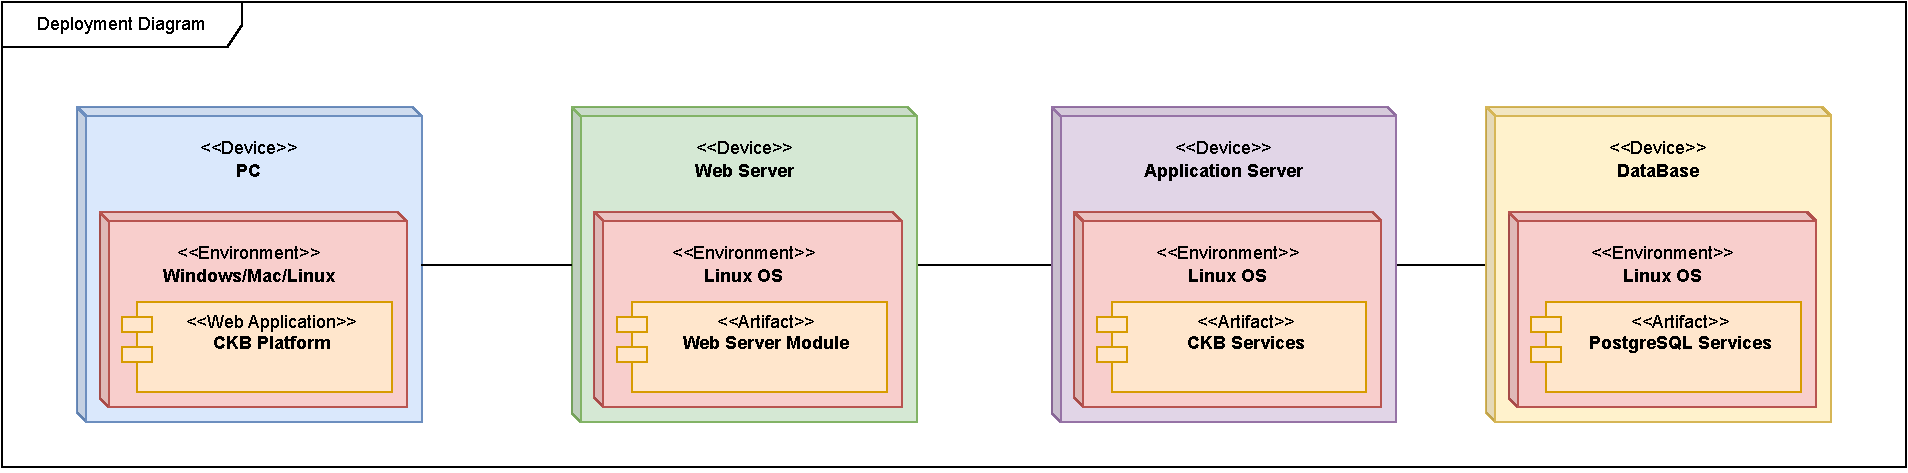
\includegraphics[scale=0.53]{images/DeploymentDiagram.pdf}
    \caption{Component diagram}
    \label{fig:deploymentDiagram}
\end{figure}

The Deployment Diagram in figure shows the components needed for the correct system behaviour. The External APIs are not included, since they 
are already implemented and found online.\\
Each device has its own operating system downloaded, the different tiers in the figure are:\\
\begin{itemize}
\item \textbf{Tier 1:} The First tier is the client tier. On the client's machine can run any OS (Windows 11 32 bit, for example) and any web browser. The web application
needs to be able to correctly run on any web browser downloaded on any OS.\\
\item \textbf{Tier 2:} The Second tier is the Web Application tier. Here no logic is found, is where the CKB platform can be accessed.
The Web Server is stored here, is contains no logic besides the bases needed for a correct execution of the website (CSS, JavaScript and Bootsrap 5.0). \\
This tier simply receives request from the client and forwards them to the Third tier, it then receives and shows the answer he received from the Third tier
 to the requesting client. \\
 \item \textbf{Tier 3:} The Third tier stores the Application Servers. The servers include all the main logic needed by the CKB platform to correctly perform.
The Third tier receives all the forwarded requests from the clients, interacts with the Fourth tier to get data, and evaluates a response. The response is 
then sent up to the Second tier, which will show the answer to the client. Each module is mapped onto this tier. This tier is the one that mainly interacts
with all external APIs. \\
\item \textbf{Tier 4:} The Fourth tier is composed by the DBMSs needed by the CKB platform for correctly interacting with the DataBases. The DBMSs function as gateways 
between the Third tier and the actual DataBases. They perform the actions requested by the Third tier and respond with the data requested.\\
\end{itemize}
\subsection{Component Interfaces}
The Component Interfaces here described are the most important ones exposed by the components.
Only the most relevant method parameters and methods are shown.
\begin{itemize}
\item \textbf{Account Manager}
    \begin{itemize}
        \item \textbf{registerUser(userData):} This method takes a data struct containing all the user's data and contacts the DBMS in order to 
        register the new user in the system. A reply is then sent to the caller.
        \item \textbf{loginUser(userData):} This method takes a data struct conntaining all the user's data, contacts the DMBS, runs a query that checks
        for the data matching the user's data provided and, if found, creates a valid session with the user's data, then logs the user in the platform.
        \item \textbf{checkUser(sessionData):} This method takes the session data and checks whether the user is a Student or and Educator.
        This method is needed and will be used by all the methods that need to show the created battles and tournaments by an Educator.
    \end{itemize}
    \item \textbf{Tournament Manager}
    \begin{itemize}
        \item \textbf{getCreatedTournaments(userId):} This method takes the user's ID from the session data, contact the DBMS which will check 
        if the user has created any tournaments and returns the json containing the new page to display, containing all the user's created tournaments.
        If no tournaments are found, the json returned will be an empty page.
        \item \textbf{createTournament(userId, tournamentData):} This method takes the user's ID and the tournament's data, which will be contained in an ad-hoc
        created struct. The method will contact the DBMS and create a new tournament with the data contained in the tournamentData. 
        The method will then return a json file containing a confirmation page.
        If any check returns negative, or the process incurs in any errors, an error message will be returned, and nothing will be inserted in the DB.
        \item \textbf{closeTournament(tournamentId, userId):} This method takes the user's ID and a tournament's ID, contacts the DBMS which will
        check if the tournament corresponding to the tournament's ID provided is created by the user with the provided user's ID, then, if the 
        check returns a positive result, updates the tournament in the database and sets its state to "closed", then returns a json containing a confirmation page.
        If the check provides a negative result, an error message will be displayed.
        \item \textbf{getSubscribedTournaments(userId):} This methods takes the user's ID, checks if the user is a Student by interacting with the DBMS and, 
        if the user is indeed a Student, returns the page containing all the tournaments he is subscribed to in json format.
        If the user is not a Student or an error occurs while interacting with the DBMS, an error page will be displayed.
        \item \textbf{enterTournament(userId, tournamentId):} This method takes the user's ID and tournament's ID and checks whether the user is a Student and if the 
        tournament is still open.
        If the user is a Student and the tournament is open, the Tournament Manager will interact with the DBMS and subscribe the provided Student to the provided tournament
        by updating the database. A confirmation page will appear after the update.
        If an error occurs while interacting with the DBMS, the user is not a Student or if the tournament is closed, an error page will be displayed.
    \end{itemize} 
    \item \textbf{Battle Manager}
    \begin{itemize}
        \item \textbf{getCreatedBattles(userId):} This method takes the user's ID from the session data, contact the DBMS which will check if the 
        user has created any battles and returns the json containing the new page to display, containing all the user's created battles. 
        If no battles are found, the json returned will be an empty page.
        \item \textbf{createBattle(userId, battleData):} This method takes the user's ID and the battle's data, which will be contained in an ad-hoc
        created struct. The Battle Manager will check if the user is an Educator through the checkUser method and if the battle will be contained in a tournament in which 
        the user's has permission to create one. If all the checks pass then the method will contact the DBMS and create a new battle with the data contained in battleData. 
        The method will then return a json file containing a confirmation page. 
        If any check returns negative, or the process incurs in any errors, an error message will be returned, and nothing will be inserted in the DB.
        \item \textbf{getSubscribedBattles(userId, tournamentId):} This methods takes the user's ID and the tournament ID,
        checks if the user is a Student and if the user is subscribed to the tournament corresponding to the given tournament ID by interacting with the DBMS and, 
        returns a page containing all the battles the user is subscribed to, contained in the tournament provided.
        If the user is not a Student or an error occurs while interacting with the DBMS, an error page will be displayed.
        \item \textbf{getBattleData(battleId, userId):} This method takes the battle's ID and the user's ID and performs a check to understand whether the 
        user is a Student or an Educator.
        If he's a Student, the returned page will contain data corresponding to the battle provided, which are deemed interesting to a Student, if he's an Educator,
        different type of data will be provided, also relative to the battle provided.
        If an error occurs while interacting with the DBMS, an error page will be provided.
        \item \textbf{enterBattle(groupId, battleId):} This method takes the group's ID and battle's ID and checks whether the group exisst, if the 
        battle is still open, if each Student in the provided group is subscribed to the tournament containing the provided battle and if the group is not already subscribed to 
        the specified battle.
        If all checks pass, the Battle Manager will interact with the Tournament DBMS and subscribe the provided group to the provided battle by updating the database. 
        A confirmation page will appear after the update.
        If an error occurs while interacting with the DBMS or any of the checks are not passed an error page will be displayed.
    \end{itemize}
    \item \textbf{Badge Manager}
    \begin{itemize}
        \item \textbf{getCreatedBadges(userId):} This method takes the user's ID from the session data, contact the DBMS which will check if the 
        user has created any badges and returns the json containing the new page to display, containing all the user's created badges. 
        If no badges are found, the json returned will be an empty page.
        \item \textbf{createBadge(userId, badgeData):} This method takes the user's ID and the badge's data, which will be contained in an ad-hoc
        created struct. The Badge Manager will check if the user is an Educator through the checkUser method and if the badge will be contained in a tournament in which 
        the user's has permission to create one. If all the checks pass then the method will contact the DBMS and create a new badge with the data contained in badgeData. 
        The method will then return a json file containing a confirmation page. 
        If any check returns negative, or the process incurs in any errors, an error message will be returned, and nothing will be inserted in the DB.
        \item \textbf{editBadge(badgeId, userId, badgeData):} This method takes the user's ID, the badge's ID and the new badge data, which will be
        contained in an ad-hoc made struct. The method then contacts the DBMS, which will check if the badge is contained in a tournament created by
        the user corresponding to the user provided, if the badge exists and, if the badge is not a tournament the user created, if the user has
        permission to edit the tournament. If each check passes, then the old badge's data will be overwritten by the new data and a json containing
        a confirmation page will be returned, else an error will be displayed.
        \item \textbf{deleteBadge(badgeId, userId, tournamentId):} This method takes the user's ID, the badge's ID and the tournament's ID and, 
        after having run checks to verify that the user has permission to delete the specified badge in the specified tournament, contacts the DBMS which will
        delete the badge from the database.
        If everything in the procedure is correct, a confirmation page will be returned, else an error page will be displayed.
        \item \textbf{checkBadges():} This method, once per day, at random intervals, cycles each group subscribed to each open battle in the platform and checks for each
        Student if they achieved any of the badges that were assigned to that battle. If the check returns positive, the Badge Manager will grant the Student his newly 
        achieved badge which will be visible on his profile.
        This method will also be invoked when a battle is closed, so that badges will be granted also on the last commits made by each group.
        \item \textbf{getBadges(userId):} This methods takes the user's ID, checks if the user is a Student by interacting with the DBMS and, 
        if the user is indeed a Student, returns all the badges he achieved while using the platform.
        If the user is not a Student or an error occurs while interacting with the DBMS, an error page will be displayed.
    \end{itemize}
    \item \textbf{Notification Manager}
    \begin{itemize}
        \item \textbf{sendGroupInvite(senderId, receiverId):} This method takes the sender's and receiver's ID, checks whether both are indeed Students, then by interfacing 
        with external Notification APIs sends a notification to the receiving Student via e-mail.
        \item \textbf{receiveInvitationAnswer(senderId, receiverId, answer):} This method takes the sender's and receiver's ID, checks whether both are indeed Students, then,
        after the Student who previously received a group invitation answers it, sends the answer to the Student who asked him to be in a group toghether via e-mail, using
        external Notification APIs.
        \item \textbf{sendTournamentNot(tournamentId):} This method takes the newly created tournament's ID and automatically sends each Student subscribed to the platform an 
        e-mail, notifying them of the creation of the new tournament, using external Notification APIs. 
        \item \textbf{sendBattleNot(battleId):} This method takes the newly created battle's ID and automatically sends each Student subscribed to the tournament containing the 
        new battle a notification, notifying them of the creation of this battle via e-mail, using external Notification APIs.
        \item \textbf{evalBattleNot(battleId, groupId):} This method is called after the computation of the "evaluate" and "editScore" methods. It takes the battle's ID and 
        the evaluated group's ID, then sends each group member a notification via e-mail, letting them know that a new score was assigned to them for their newly
        uploaded solution. This is achieved using external Notification APIs.
    \end{itemize}
    \item \textbf{Evaluation Manager}
    \begin{itemize}
        \item \textbf{editScore(battleId, userId, score, studentID):} This method takes the user's ID, the battle's ID, the Student's ID and the new score to assign to the 
        corresponding Student for the corresponding battle. The method checks if the user has permission to edit the Student's grade in the corresponding battle and, 
        if he can, will then contact the DBMS and update the Student's old grade with the new one provided for the specified battle. 
        A confirmation page will be sent back to the user.
        If the platform runs into any error in the process, or if the user doesn't have the necessary permissions, an error page will be displayed, and the database will not be
        updated.
        \item \textbf{evaluate(battleId, groupId):} This method takes the battle's ID and the group's ID, then performs a search to find the tests written to automatically
        evaluate the battle provided, runs them on the group's provided solution and assigns each group member a grade on a scale from 0 to 100.
        The grade will be automatically generated based on the test creator previously specified data.
        \item \textbf{getScore(battleId, groupId):}  This method takes the battle's ID and the group's ID and returns the latest score assigned to the provided group for the 
        specified battle. If no score is found, a score of 0 will be automatically returned.
    \end{itemize}
    \item \textbf{Group Manager}
    \begin{itemize}
        \item \textbf{createGroup(studentId, invitedIds):} This method takes the provided Student's ID and an array of the invited Students' IDs, checks if each ID corresponds
        to a Student's id saved in the platform and, if so, creates the group, saving it in the group's database.  
    \end{itemize}
\end{itemize}
\subsection{Runtime view}
    \subsubsection{Student sign-up to the platform}
        \begin{figure}[H]
            \centering
            \hspace*{-2cm}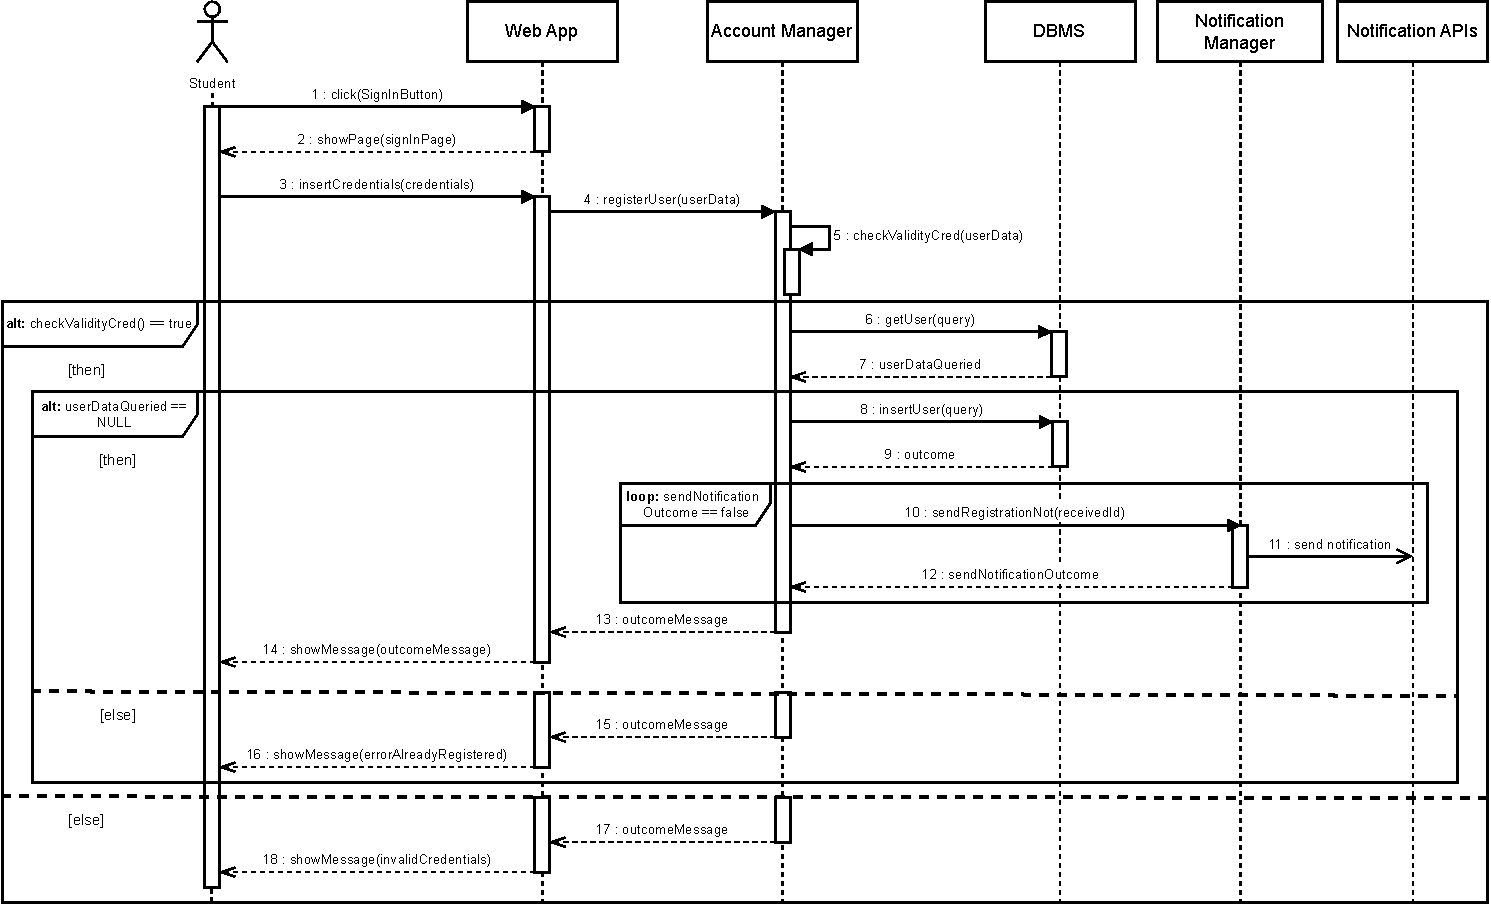
\includegraphics[scale=0.65]{Sequence/Sequence1DD.pdf}
            \caption{Sign-up sequence diagram}
            \label{fig:Sequence1DD}
        \end{figure}

        The above diagram represents the process of a Student's signing up.
        The Student accesses to the CKB platform WebApp Homepage through their browser
        (omitted for simplicity). They then clicks on the "SIGN IN" button as
        shown in figure \ref{fig:homepageMockup}. The WebApp will show a form
        which the Student has to fill with their informations such as
        name, surname, username that want to use in the platform, email,
        password, attended school, ... 
        \\ \\
        Once the Student confirms the registration the WebApp contacts the
        Account Manager which evaluates the request.
        The Account Manager is in charge of checking the validity of the Student's credentials,
        i.e. checking whether the name, surname or username inserted by the Student
        contains some not acceptable characters for some reason, the password
        don't respects security standards, ... \\
        Other than that the Account Manager takes care to verify if the Student is already
        registered, i.e. if the used email already appears in the DB. This is done by interfacing
        with the DBMS.
        \\ \\
        At this point we can have three possible situations:
        \begin{enumerate}
            \item \textbf{Credentials validation went wrong:} In this case the WebApp will show to the
            Student an error message of invalid credentials
            \item \textbf{Student has already registered with the same email:} In this case the WebApp will show to the
            Student an error message stating that they have already registered.
            \item \textbf{Valid credentials and email used for the first time:} In this case the Account
            Manager proceeds to communicate to the DBMS to insert the Student's data in the DB.
            Proceeds to inform the Notification Manager to send an email of confirmation for the registration.
            Finally returns the positive outcome of the operation to the WebApp, which in 
            turn will show a confirmation message to the Student.
        \end{enumerate}

    \subsubsection{Educator sign-up to the platform}
        \begin{figure}[H]
            \centering
            \hspace*{-2.2cm}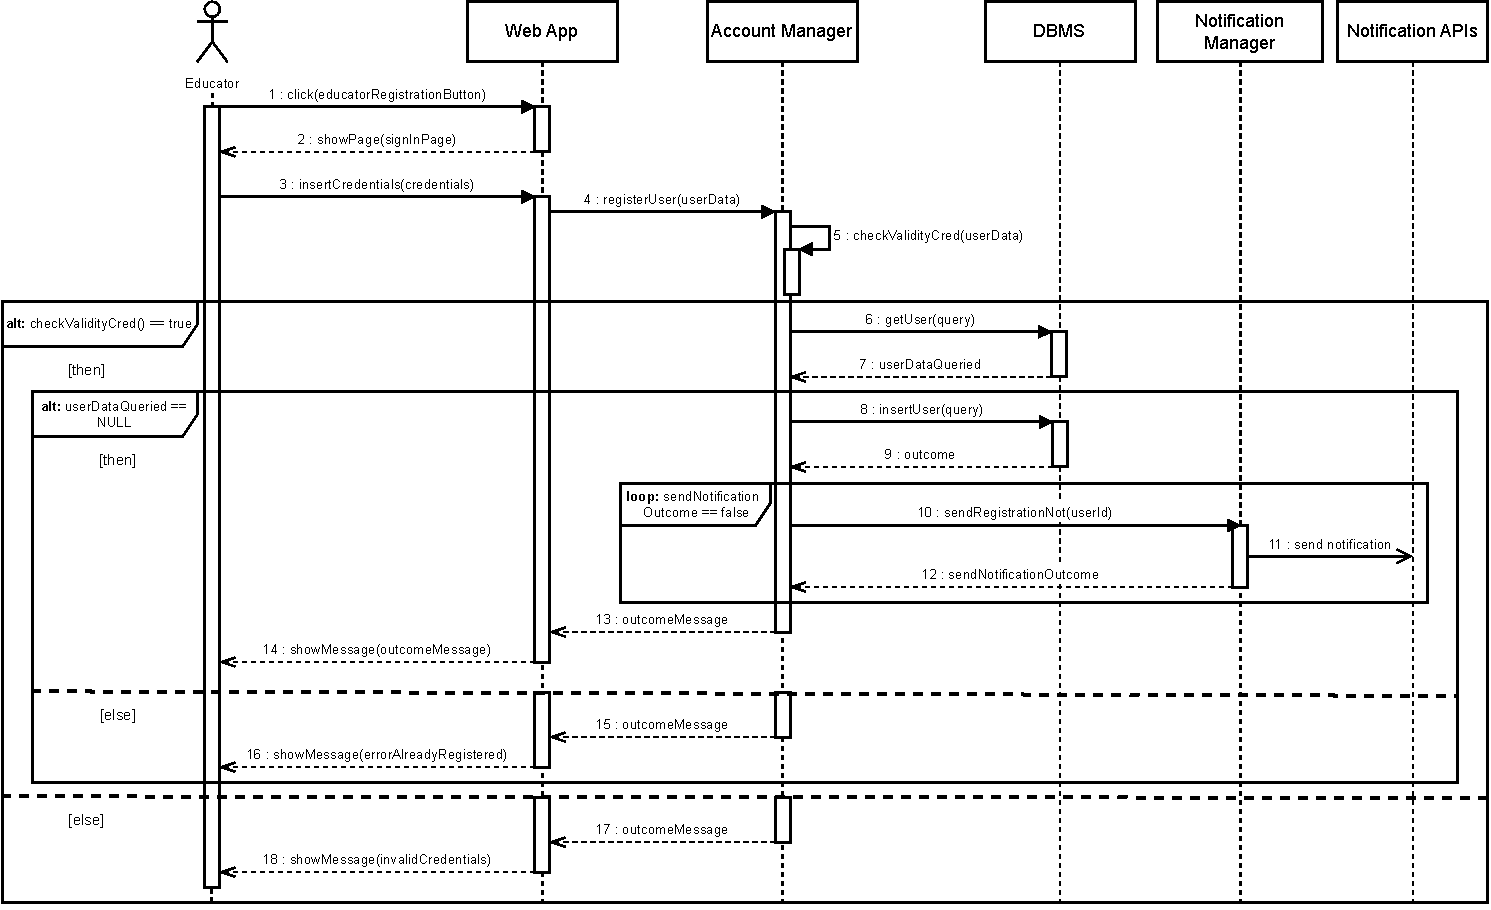
\includegraphics[scale=0.65]{Sequence/Sequence2DD.pdf}
            \caption{}
            \label{fig:Sequence2DD}
        \end{figure}

        The above diagram, represents the process of an Educator's signing up.
        The process is pratically identical to the Student's one with the exception of the
        data that the Educator is requested to insert in the form, such as their name, surname
        username, school in which they teaches, istitutional email, password, ... 

    \subsubsection{Educator creates a new tournament}
        \begin{figure}[H]
            \centering
            \hspace*{-4cm}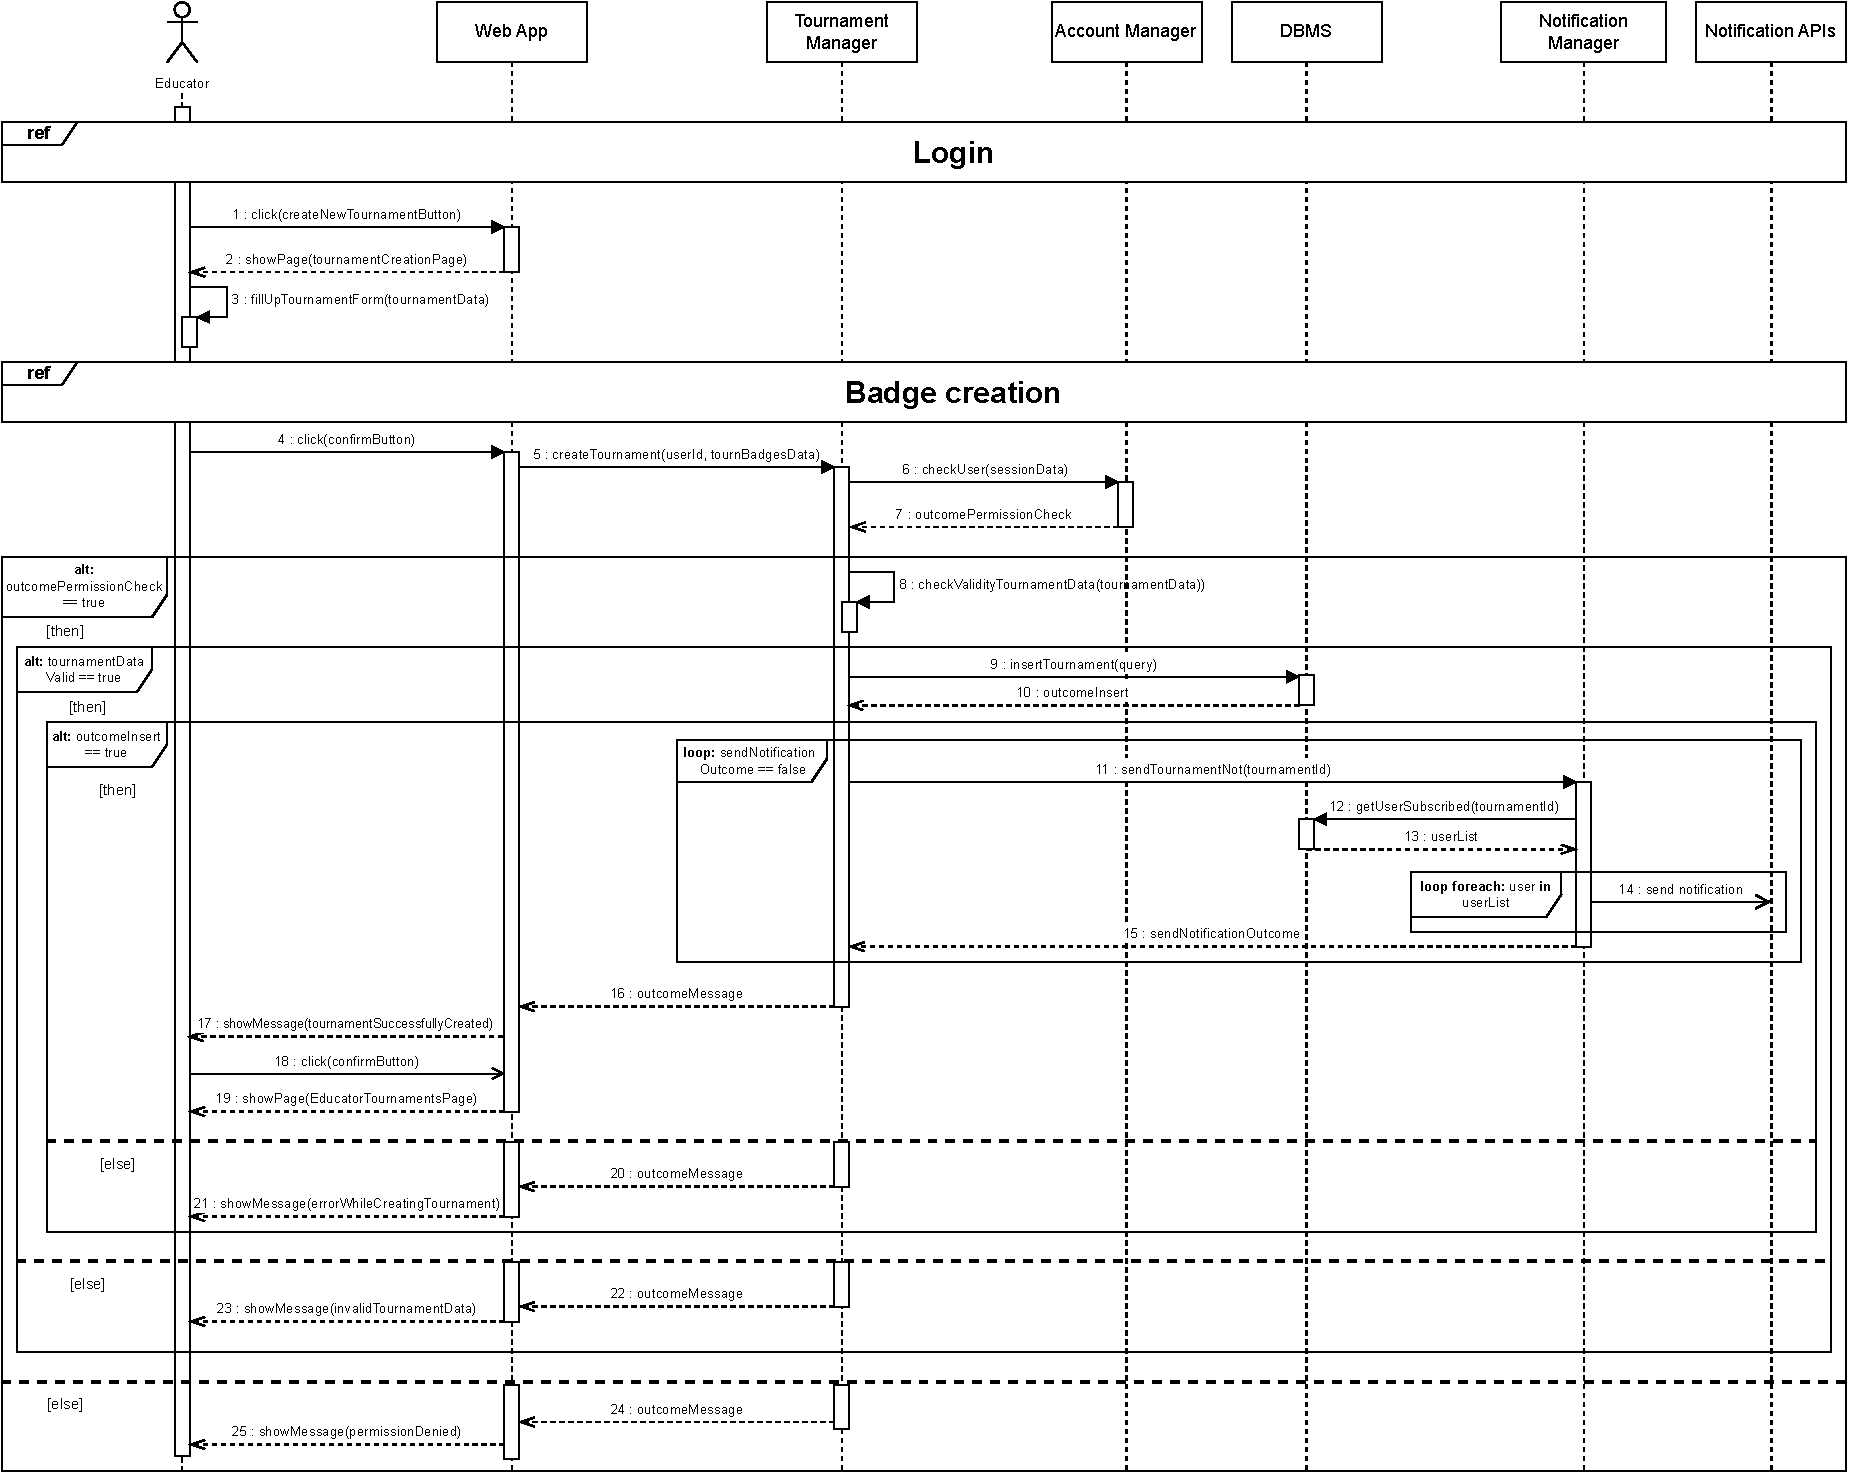
\includegraphics[scale=0.65]{Sequence/Sequence3DD.pdf}
            \caption{}
            \label{fig:Sequence3DD}
        \end{figure}

        The above diagram represents the tournament's creation by an Educator.
        In order to start this process the Educator must have completed the login procedure
        first, as shown in \ref{fig:loginSequence} figure.
        The Educator has to access to the riepilogative page of their tournaments 
        (this part of the process was omitted for simplicity) and here, they have to click 
        on the "Create new Tournament" button (as shown in \ref{fig:tournamentsPage}).
        The WebApp will show a Tournament creation page (\ref{fig:tournamentCreationPage})
        in which there is a form that the Educator has to fill.
        At this point the Edcuator can creates new badges to insert in the tournament. This
        process is displayed in the Sequence Diagram 2.5.4 \ref{fig:Sequence4DD}

    \subsubsection{Educator creates new badges}
        \begin{figure}[H]
            \centering
            \hspace*{-1cm}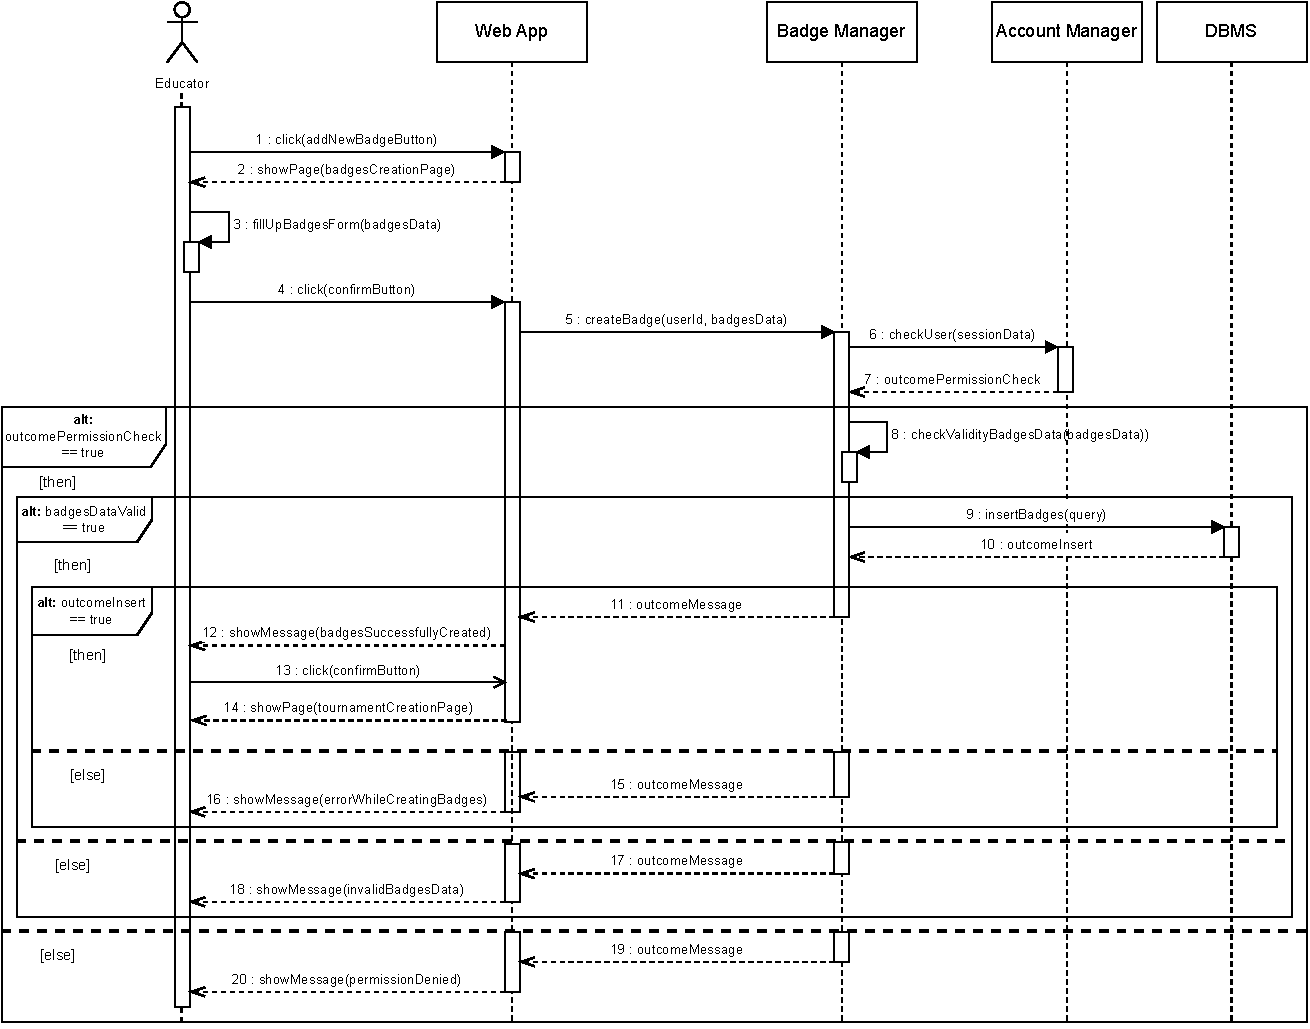
\includegraphics[scale=0.65]{Sequence/Sequence4DD.pdf}
            \caption{}
            \label{fig:Sequence4DD}
        \end{figure}
    \subsubsection{Educator deletes and/or updates a badge}
        \begin{figure}[H]
            \centering
            \hspace*{-0.7cm}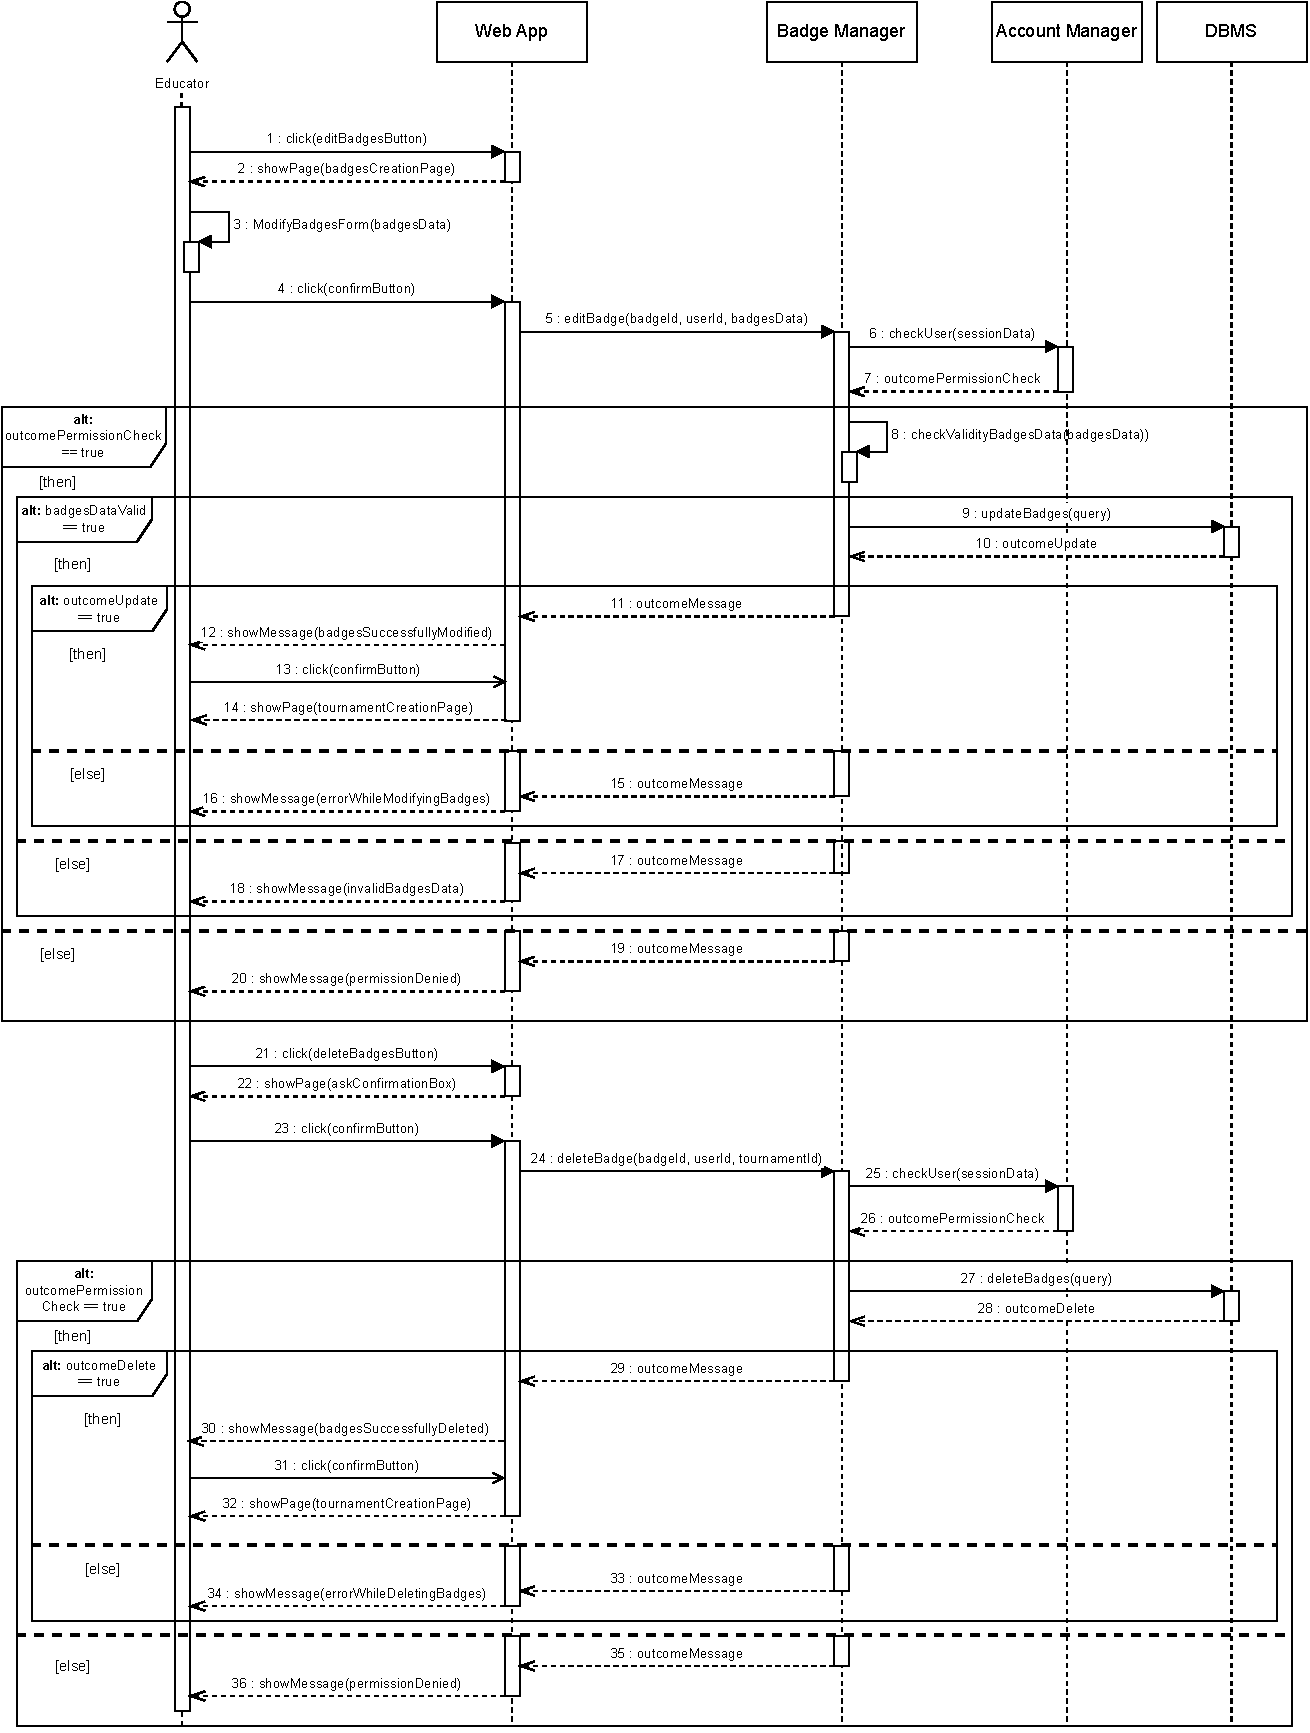
\includegraphics[scale=0.60]{Sequence/Sequence5DD.pdf}
            \caption{}
            \label{fig:Sequence5DD}
        \end{figure}
    \subsubsection{Educator creates a new battle}
        \begin{figure}[H]
            \centering
            \hspace*{-3.1cm}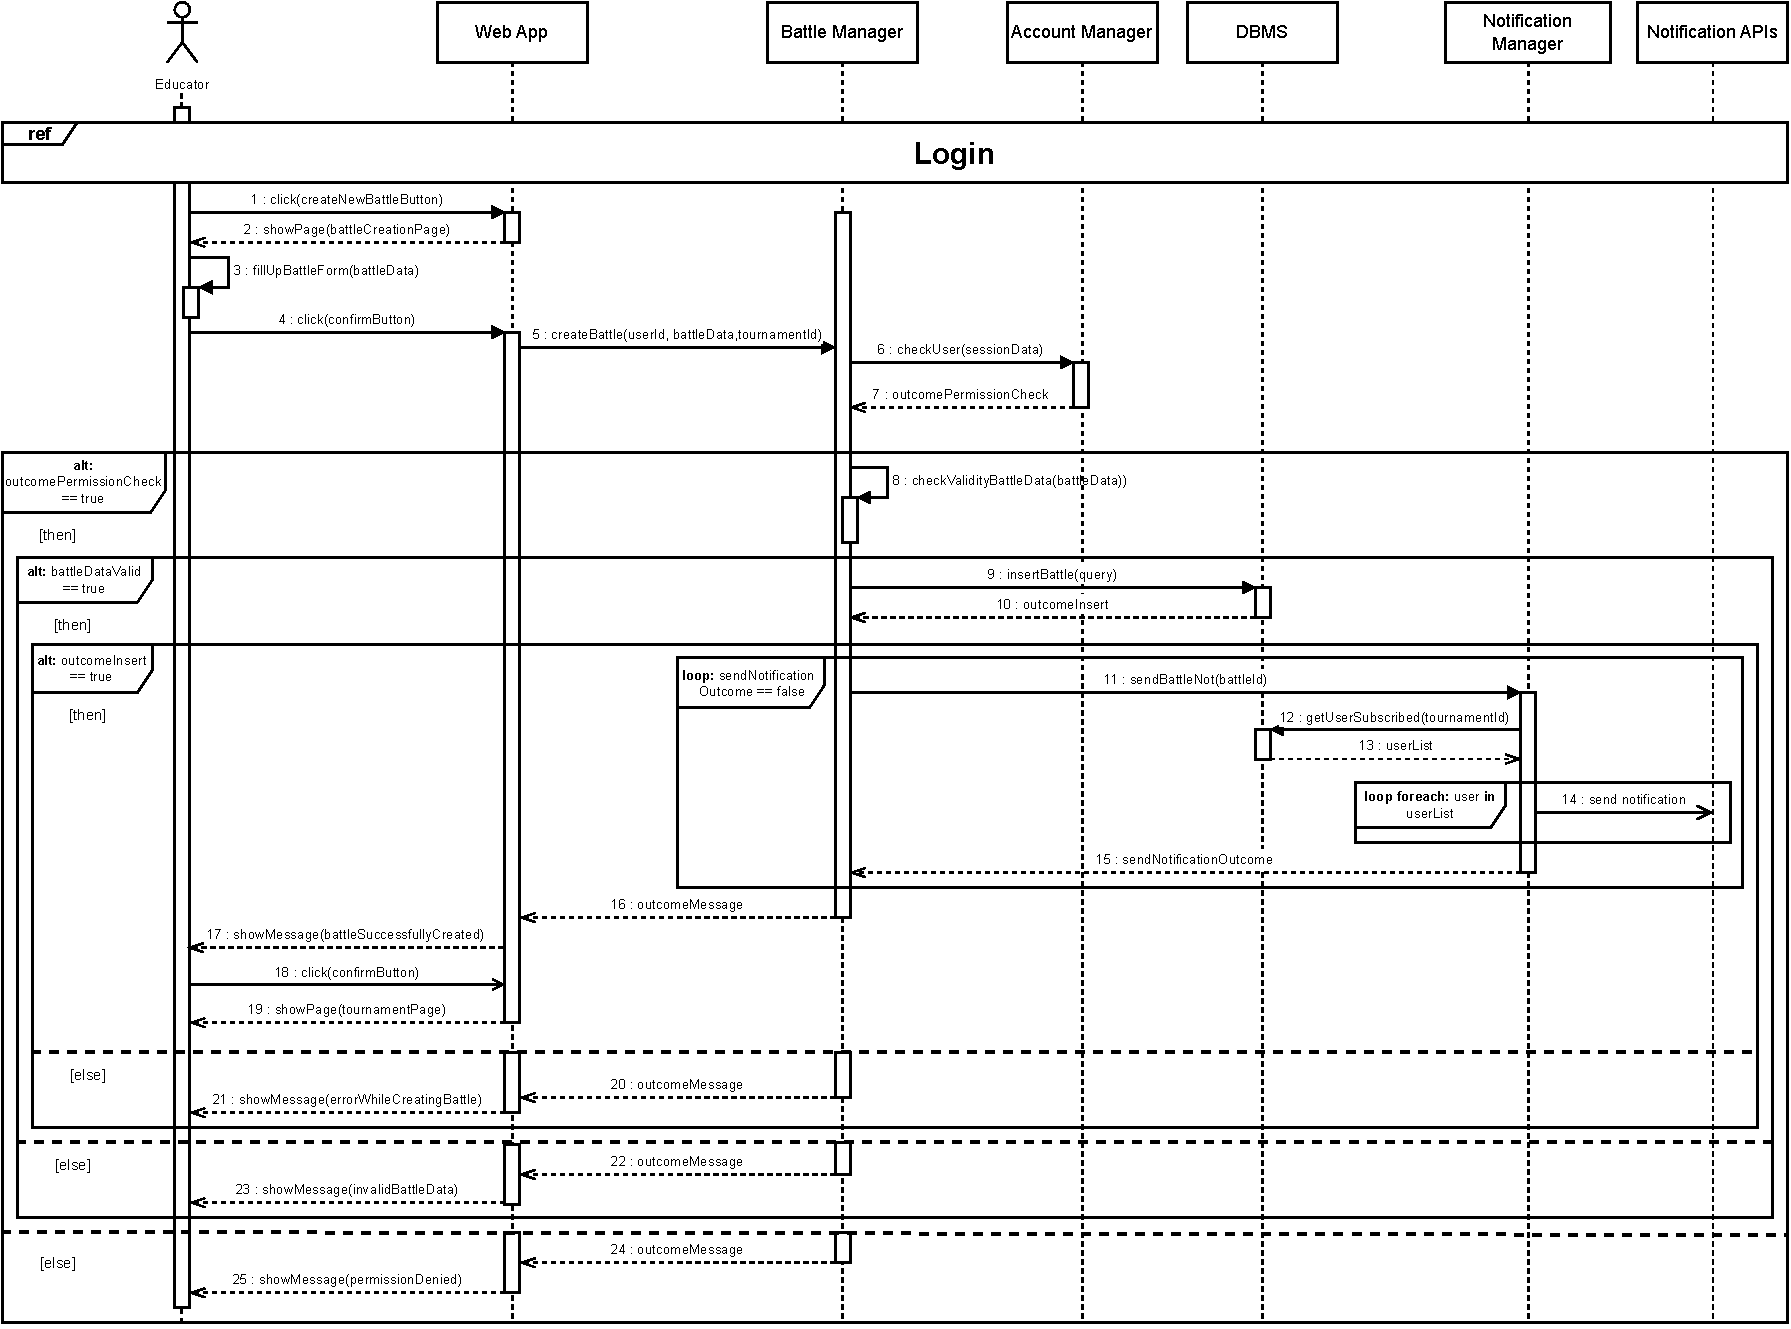
\includegraphics[scale=0.6]{Sequence/Sequence6DD.pdf}
            \caption{}
            \label{fig:Sequence6DD}
        \end{figure}

        The above diagrams represents the process of creating a new battle within a tournament,
        by an Educator. \\
        The Educator accesses to the CKB platform WebApp Homepage and subsequently
        to the page of one of the tournaments they have created, all of this through their browser
        (omitted for simplicity).
        They then click on the "Create new Battle" button as shown in figure \ref{fig:tournamentManagementPage}.
        \\ \\
        The WebApp will show a page which will contains a form that the Educator can fill with
        the battle's data, such as its name, maximum and minumum number of member per group,
        registration and submission deadlines, programming language accepted, ... 
        \\ \\
        Once the Educator press the "Confirm" button (as shown in figure \ref{fig:battleCreationPage})
        the battle's data will be sent to the Battle Manager. \\
        The Battle Manager will contacts the Account Manager, to verify, through the session's 
        data, whether the logged Educator has the permissions to create a new battle within that 
        tournament. 
        If that's the case then the Battle Manager will check the validity of the battle's data 
        inserted, i.e. checking whether one or more data don't respect some standards.
        \\ \\
        If the check succeeds then the Battle Manager will try to insert the battle in the DB,
        by contacting the DBMS. \\
        If the insertion succeeded then the Battle Manager will interfaces with the Notification
        Manager which will send the notification of the battle's creation to all the Student
        subscribed to the tournament (N.B. The notification manager will continuosly trying to
        send notification if their SUBMISSION fails server side for some reasons, it will NOT
        try to resend them if the receivers don't receive them). 
        In the meantime the Battle Manager component will return a message of success to 
        the Educator through the WebApp.
        \\ \\
        There are several cases in which this process won't succeeds. In order we have:
        \begin{itemize}
            \item \textbf{Educator does not have permissions:} In case the Educator is not the 
            tournament's creator or has not been granted access to it from another collegue, 
            the Battle Manager will return an error message stating that the the procedure was 
            denied. 
            The message will be shown by the WebApp to the Educator themselves.
            \item \textbf{Battle's data are invalid} In this case after the check, the Battle 
            Manager component just return an error message to the WebApp stating that the 
            inserted data were not valid. The message will then be shown to the Educator by 
            the WebApp.
            \item \textbf{Battle's insertion in the DB went wrong:} In this case no 
            notification will be sent to the Students, and the Battle Manager component will 
            return to the WebApp an error message stating that there was an error while 
            creating the battle.
            The message will then be shown by the WebApp to the Educator.
        \end{itemize}


    \subsubsection{Educator closes a tournament}
        \begin{figure}[H]
            \centering
            %\hspace*{-3.7cm}\includegraphics[scale=0.65]{}
            \caption{}
            \label{fig:}
        \end{figure}
    \subsubsection{Educator evaluates a battle's results}
        \begin{figure}[H]
            \centering
            %\hspace*{-3.7cm}\includegraphics[scale=0.65]{}
            \caption{}
            \label{fig:}
        \end{figure}
    \subsubsection{Student forms a group}
        \begin{figure}[H]
            \centering
            %\hspace*{-3.7cm}\includegraphics[scale=0.65]{}
            \caption{}
            \label{fig:}
        \end{figure}
    \subsubsection{Student joins a battle}
        \begin{figure}[H]
            \centering
            %\hspace*{-3.7cm}\includegraphics[scale=0.65]{}
            \caption{}
            \label{fig:}
        \end{figure}
    \subsubsection{Student uploads a new solution}
        \begin{figure}[H]
            \centering
            %\hspace*{-3.7cm}\includegraphics[scale=0.65]{}
            \caption{}
            \label{fig:}
        \end{figure}
    \subsubsection{Student uploads a solution after submission deadline}
        \begin{figure}[H]
            \centering
            %\hspace*{-3.7cm}\includegraphics[scale=0.65]{}
            \caption{}
            \label{fig:}
        \end{figure}
    \subsubsection{Student visualizes his tournament's results and badges}
        \begin{figure}[H]
            \centering
            %\hspace*{-3.7cm}\includegraphics[scale=0.65]{}
            \caption{}
            \label{fig:}
        \end{figure}
\subsection{Selected architectural styles and patterns}
    \subsubsection{Four-layered architecture:} We chose this architecture for many reasons, mainly:
    \begin{itemize}
        \item \textbf{Maintainability:} By having four different layers, with separated logic and data, once the platform's structure is fully defined
        each layer's interior logic will be fully defined.
        By having separated logic and data, it will be easier in the future to access and solve possible problems that can occur in different 
        layers.
        \item \textbf{Security:} By separating the web, application and data servers in different internet partition divided by firewalls, we create multiple
        DMZs, resulting in a more secure architecture. Before accessing the data layer, a malicious user would need to surpass three different firewalls. 
    \end{itemize}
    \subsubsection{MicroServices architecture:} The MicroServices architecture is what we chose since the platform will be developed as a collection of 
    services. MicroServices are needed for a fast, modern and reliable system, since what we want to achieve here is dividing each task in multiple, 
    smaller ones, that are easier to work with.
    We chose the MicroServices architecture to ensure these properties in the system:
    \begin{itemize}
        \item \textbf{Load Distribution:} The presence of multiple application servers and databases assures us that the platform will be fast 
        and reliable in all its elaborations. If we didn't have load balancing or any sort of redundancy we would have found ourselves with multiple
        single nodes having to serve multiple requests, causing overloading and possible deadly failures.
        \item \textbf{Scalability:} The result of load distribution ensures that redundancy is provided only for the most important parts of the platform.
        This ensures maximum scalability with minimal cost.
    \end{itemize}
    \subsubsection{REST architecture:}
    The REST architecture is a set of rules to follow while building a web application, to ensure that the web application being built is stateless.
    This means that the server does not care about the client's status information, but those informations are dealt with by the client.
    \begin{itemize}
    \item \textbf{Cacheability:} For a web application to be RESTFul, it needs to be cacheable. Having a web cache makes the web application much faster when handling 
    requests, since the application servers will not be accessed each time a request is made. Instead, cache proxies present in the network will parse the requests and
     answer for them, if the data they have is not too old.
    \item \textbf{Uniform interface:} Having uniform interfaces thoughout all its users, the web application ensures that it can be accessed from any browser, downloaded
    on any operating system. This is an important constraint, as any user can access and use the CKB platform.
    \end{itemize}
\subsection{Other design decisions}
    \subsubsection{Relational Database:} We chose to implement our databases in a relational way, since relational databases are the go-to choice when 
    implementing a web application. Relational databases are needed when we want to ensure that data will not be lost in time and we want data to be kept sure.
    Since we want to implement our web application following the MicroServices architectural style, we chose to separate our data in three different databases.
    We have a database dedicated only to the users' data, containing all the different users. This database is accessed on login, registration and when the 
    session is created.
    We have a database dedicated to the tournaments' data, containing all battles, badges and tournaments. This database is accessed each time a request 
    is made that needs to access or modify some data related to tournaments.
    We have a database dedicated to Students' groups, accessed each time a new group is created.
    Each database is developed using the PostgreSQL language, since it has a better trigger architecture than MySQL or MariaDB.
\section{User Interface Design}
\section{Requirements traceability}
\begin{itemize}
    \item \textbf{R.1:} The CKB platform should allow an
        unregistered Student to create a new account.
        \begin{itemize}
            \item \textbf{User Database:} Used to store Students' informations after registration.
        \end{itemize}
    \item \textbf{R.2:} The CKB platform should allow an
        unregistered Educator to create a new account.
        \begin{itemize}
            \item \textbf{User Database:} Used to store Educators' informations after registration.
        \end{itemize}
    \item \textbf{R.3:} The CKB platform must allow access to its pages only if the used credentials are correct.
        \begin{itemize}
            \item \textbf{Account Manager:} Used to check whether the credentials used are correct.
            \item \textbf{Account Manager:} Used to retrieve users' data.
        \end{itemize}
    \item \textbf{R.4:} The CKB platform must not allow a Student to register more than once in the system.
          \begin{itemize}
              \item \textbf{Account Manager:} Used to check if the Student has 
              already registered to the platform.
              \item \textbf{Account Manager:} Used to retrieve Student's data.
          \end{itemize}
    \item \textbf{R.5:} The CKB platform must not allow an Educator to register more than once in the system.
          \begin{itemize}
              \item \textbf{Account Manager:} Used to check if the Educator has already
              registered to the platform.
              \item \textbf{Account Manager:} Used to retrieve Educator's data.
          \end{itemize}
    \item \textbf{R.6:} Educators can access the platform's services only if they are registered to it.
          \begin{itemize}
              \item \textbf{Account Manager:} Used to check if the Educator is registered to
              the platform.
              \item \textbf{Account Manager:} Used to retrieve Educator's data.
          \end{itemize}
    \item \textbf{R.7:} Students can access the platform's services only if they are registered to it.
          \begin{itemize}
            \item \textbf{Account Manager:} Used to check if the Student is registered to
            the platform.
            \item \textbf{Account Manager:} Used to retrieve Student's data.
          \end{itemize}
    \item \textbf{R.8:} The CKB platform should not allow Students to create tournaments and/or battles.
          \begin{itemize}
              \item \textbf{Account Manager:} Used to check if the user is a Student and prevent him
              to access Tournament Manager APIs that should not have access to.
              \item \textbf{Account Manager:} Used to retrieve Student's data.
          \end{itemize}
    \item \textbf{R.9:} The CKB platform should allow Educators to create battles within a tournament only to the tournament
          creator and to any other Educator that has been granted permission to do so by the tournament creator.
          \begin{itemize}
              \item \textbf{Account Manager:} Used to check whether the logged Educator can create
              a battle within a certain tournament.
              \item \textbf{Battle Manager:} Used to create the new battle within the tournament.
              \item \textbf{Account Manager:} Used to retrieve Educator's data. 
              \item \textbf{Tournament Database:} Used to store the newly created battle's data.
          \end{itemize}
    \item \textbf{R.10:} The CKB platform must allow Educators to personalise the tournaments they create.
          \begin{itemize}
              \item \textbf{Tournament Manager:} Used to create and personalize new tournaments.
              \item \textbf{Tournament Database:} Used to store tournament's data.
          \end{itemize}
    \item \textbf{R.11:} The CKB platform must allow Educators to personalise the battles they create.
          \begin{itemize}
              \item \textbf{Battle Manager:} Used to create and personalize new battles.
              \item \textbf{Tournament Database:} Used to store battle's data.
          \end{itemize}
    \item \textbf{R.12:} The CKB platform must allow Educators to define new obtainable badges for each tournament they
          create.
          \begin{itemize}
              \item \textbf{Badges Manager:} Used to create new badges for a new tournament.
              \item \textbf{Tournament Database:} Used to store badges data.
          \end{itemize}
    \item \textbf{R.13:} The CKB platform must allow Educators to manually evaluate the solutions uploaded by the Students for the battles that
          the Educators created.
          \begin{itemize}
              \item \textbf{Battle Manager:} Used to check whether the battle is enabled to be manually
              evaluated.
              \item \textbf{Evaluation Manager:} Used to allow the Educator to manually evaluate Students'
              work.
              \item \textbf{Account Manager:} Used to retrieve Educator's data.
              \item \textbf{Tournament Database:} Used to store battle and scores' data. The scores are both the automatically generated ones and the ones
              given by the Educator through the manual evaluation process.  
          \end{itemize}
    \item \textbf{R.14:} The CKB platform must allow Educators to delete or update badges before finalizing a tournament's creation.
          \begin{itemize}
              \item \textbf{Badges Manager:} Used to update or delete some badges during tournament creation.
              \item \textbf{Tournament Manager:} Used to retrieve old badges's data.
              \item \textbf{Tournament Database:}  Used to store the badge's data.
          \end{itemize}
    \item \textbf{R.15:} The CKB platform must allow Educators to define rules to obtain badges in tournaments created by them.
          \begin{itemize}
              \item \textbf{Badges Manager:} Used to define the rules to obtain the badges.
              \item \textbf{Tournament Database:} Used to store badges's obtaining rules.
          \end{itemize}
    \item \textbf{R.16:} The CKB platform must ensure that badges' characteristics respect guidelines regarding their
          name, icon format and rules to obtain them.
          \begin{itemize}
              \item \textbf{Badges Manager:} Used to check if the characteristics of the new badges
              that the Educator wants to create, or the modifications made to the ones already 
              created, respect some constraints.
          \end{itemize}
    \item \textbf{R.17:} The CKB platform must allow Educators to create new tournaments.
          \begin{itemize}
              \item \textbf{Tournament Manager:} Used to create new tournaments.
              \item \textbf{Tournament Database:} Used to store tournament's data.
          \end{itemize}
    \item \textbf{R.18:} The CKB platform must ensure that tournaments' characteristics respect guidelines regarding their
          name, deadline, access method, programming language.
          \begin{itemize}
              \item \textbf{Tournament Manager:} Used to check if the characteristics of the tournaments
              that the Educator wants to create respect some constraints.
          \end{itemize}
    \item \textbf{R.19:} The CKB platform must allow Educators to close tournaments they have created.
          \begin{itemize}
              \item \textbf{Tournament Manager:} Used to allow Educators to close the tournaments that they have
              created.
              \item \textbf{Tournament Manager:} Used to retrieve old tournament's data.
              \item \textbf{Tournament Database:} Used to store tournaments' data.
          \end{itemize}
    \item \textbf{R.20:} The CKB platform must ensure that when a tournament is closed, Educators cannot create new battles
          within it.
          \begin{itemize}
              \item \textbf{Tournament Manager:} Used to prevent Educators to create new battles
                within closed tournaments.
            \item \textbf{Battle Manager:} Used to try to create a new battle.
            \item \textbf{Tournament Manager:} Used to retrieve the data of the tournament in which
            the Educator wants to create a new battle. 
          \end{itemize}
    \item \textbf{R.21:} The CKB platform must ensure that if a group uploads a solution to a battle after the submission's deadline,
          that solution will not be considered in the score computation by preventing its upload.
          \begin{itemize}
              \item \textbf{Battle Manager:} Used to check if the submission phase of the battle has ended.
              \item \textbf{Tournament Manager:} Used to retrieve battle's data. 
          \end{itemize}
    \item \textbf{R.22:} The CKB platform must ensure that the score given to a group in a tournament is
          coherent with scores given to the same group in the battles they have partecipated in.
          \begin{itemize}
              \item \textbf{Evaluation Manager:} Used to automatically evaluate Students' uploads,
              give them a score and subsequently update Students' tournament score.
              \item \textbf{Tournament Database:} Used to store Students's scores.
          \end{itemize}
    \item \textbf{R.23:} The CKB platform must ensure fair competition between group scores. In the tournament's evaluation, the final
          group score should be the average score of all the battles in the tournament for each group. Any battle with no solution submitted will count
          as 0 points.
          \begin{itemize}
            \item \textbf{Evaluation Manager:} Used to automatically evaluate Students' uploads.
            In case of no upload by a group assigns to them 0 points.
            \item \textbf{Tournament Database:} Used to store Students's scores.
          \end{itemize}
    \item \textbf{R.24:} The CKB platform must allow Students to subscribe to a tournament.
          \begin{itemize}
              \item \textbf{Tournament Manager:} Used to allow Students to register to a tournament.
              \item \textbf{User Database:} Used to store registrations' data.
          \end{itemize}
    \item \textbf{R.25:} The CKB platform must allow Students to subscribe to a tournament's battle
          within the registration deadline.
          \begin{itemize}
              \item \textbf{Battle Manager:} Used to allow Students to register to a battle if the
              registration deadline has not expired yet.
              \item \textbf{Tournament Manager:} Used to retrieve battle's data.
              \item \textbf{Tournament Database:} Used to store Student's registration to the battle.
          \end{itemize}
    \item \textbf{R.26:} The CKB platform must allow Students to submit solutions to a tournament's battle
        within the battle's deadline relying on the external GitHub service.
          \begin{itemize}
              \item \textbf{Evaluation Manager:} Used to retrieve group's solution from GitHub.
              \item \textbf{Tournament Database:} Used to store solution's data.
          \end{itemize}
    \item \textbf{R.27:} The CKB platform must allow Students to send and receive group invitations to and from
          other Students in order to form groups.
          \begin{itemize}
              \item \textbf{Group Manager:} Used to search Students and send them invitations to groups.
              \item \textbf{Notification Manager:} Takes care of sending emails to the invited Students.
              \item \textbf{Account Manager:} Used to retrieve Students' data.
              \item \textbf{Group Database:} Used to store invitation and group's data.
          \end{itemize}
    \item \textbf{R.28:} The CKB platform should allow Students to join a battle only if the group composition rules
          for that battle are complied with.
          \begin{itemize}
              \item \textbf{Battle Manager:} Used to check whether the group that is trying to
              access the battle is violating some battle's rules, if not allows it to register to
              the battle.
              \item \textbf{Tournament Manager:} Used to retrieve battle's data.
              \item \textbf{Tournament Database:} Used to store battle registration's data.
          \end{itemize}
    \item \textbf{R.29:} The CKB platform must ensure that solutions uploaded by a Student for a battle are evaluated.
          \begin{itemize}
              \item \textbf{Evaluation Manager:} Used to evaluate solutions uploaded on GitHub by Students.
              \item \textbf{Tournament Database:} Used to store Students' scores.
          \end{itemize}
    \item \textbf{R.30:} The CKB platform must ensure that only the latest solution uploaded by a Student for a battle he is subscribed to will
          be taken into consideration for the final score.
          \begin{itemize}
              \item \textbf{Evaluation Manager:} Used to evaluate the last solution uploaded and
              overwrite Students' score according to it.
              \item \textbf{Tournament Database:} Used to store Students' scores and new solutions' data.
          \end{itemize}
    \item \textbf{R.31:} The CKB platform must allow groups partecipating in a battle to change their solution,
          if the battle's submission deadline hasn't expired yet.
          \begin{itemize}
            \item \textbf{Evaluation Manager:} Used to retrieve latest group's solution from GitHub and evaluate it.
              \item \textbf{Tournament Database:} Used to store Students' scores and new solutions' data.
          \end{itemize}
    \item \textbf{R.32:} The CKB platform must allow an Educator to modify the score for a Student's solution.
          \begin{itemize}
              \item \textbf{Evaluation Manager:} Used to allow an Educator to manually evaluate Students'
              work and change their score.
              \item \textbf{Tournament Manager:} Used to retrieve of Students' work and score.
              \item \textbf{Tournament Database:} Used to and store Studentd' scores.
          \end{itemize}
    \item \textbf{R.33:} The CKB platform must ensure that when a new tournament is created, all
          Students subscribed to the platform are going to receive a notification.
          \begin{itemize}
              \item \textbf{Notification Manager:} Used to send a notification to all the Students
              registered to the platform.
              \item \textbf{Account Manager:} Used to retrieve Students' data.
          \end{itemize}
    \item \textbf{R.34:} The CKB platform must ensure that when a new battle is created in a tournament,
          all Students subscribed to that tournament are going to receive a notification.
          \begin{itemize}
              \item \textbf{Notification Manager:} Used to send a notification to all the Students
              registered to the tournament in which the battle will take place.
              \item \textbf{Account Manager:} Used to retrieve Students' data.
          \end{itemize}
    \item \textbf{R.35:} The CKB platform must allow Students to visualise the score they obtained in a battle they partecipated in.
          \begin{itemize}
              \item \textbf{Battle Manager:} Used to allow Students access the score obtained
              in a battle they partecipated to.
              \item \textbf{Tournament Manager:} Used to retrieve battle's data and specifically
              Student's results in it.
          \end{itemize}
    \item \textbf{R.36:} The CKB platform must allow Students to visualise the score they obtained in a tournament they partecipated in.
          \begin{itemize}
            \item \textbf{Tournament Manager:} Used to allow Students access the score obtained
            in a tournament they partecipated to.
            \item \textbf{Tournament Manager:} Used to retrieve tournament's data and specifically Student's results in it.
          \end{itemize}
    \item \textbf{R.37:} The CKB platform must allow Students to visualise the badges they obtained.
          \begin{itemize}
              \item \textbf{Account Manager:} Used to allow Students to access their, or others'
              profile pages and visualize the badges in it.
              \item \textbf{Account Manager:} Used to retrieve Student's data.
          \end{itemize}
    \item \textbf{R.38:} The CKB platform must ensures that battles' characteristics respect guidelines
          regarding their name, deadlines, programming language, number of member per group.
          \begin{itemize}
            \item \textbf{Tournament Manager:} Used to check if the characteristics of the battles
              that the Educator want to create, respect some constraints.
          \end{itemize}
\end{itemize}
\section{Implementation, Integration \& Test plan}


\newpage
\section{Effort Spent}
\begin{tabular}{|g|c|c|}
    \hline
    \multicolumn{2}{|g|}{\textbf{Group member}} & \multicolumn{1}{|g|}{\textbf{Effort spent}} \\
    \hline
    \textbf{Francesco Spangaro}                 & \makecell[l]{                               \\Introduction\\Architectural Design\\User Interface Design\\Requirement Traceability\\Implementation, Integration and Test plan\\
    \vspace{\baselineskip}}                     & \makecell[l]{\textit{Xh}                    \\\textit{Xh}\\\textit{Xh}\\\textit{Xh}\\\textit{Xh} \vspace{\baselineskip}}\\
    \hline
    \textbf{Luca Tosetti}                       & \makecell[l]{                               \\Introduction\\Architectural Design\\User Interface Design\\Requirement Traceability\\Implementation, Integration and Test plan\\
    \vspace{\baselineskip}}                     & \makecell[l]{\textit{Xh}                    \\\textit{Xh}\\\textit{Xh}\\\textit{Xh}\\\textit{Xh}}\\
    \hline
    \textbf{Francesco Riccardi}                 & \makecell[l]{                               \\Introduction\\Architectural Design\\User Interface Design\\Requirement Traceability\\Implementation, Integration and Test plan\\
    \vspace{\baselineskip}}                     & \makecell[l]{\textit{Xh}                    \\\textit{Xh}\\\textit{Xh}\\\textit{Xh}\\\textit{Xh} \vspace{\baselineskip}}\\
    \hline
\end{tabular}
\section{References}




\end{document}
